% Options for packages loaded elsewhere
\PassOptionsToPackage{unicode}{hyperref}
\PassOptionsToPackage{hyphens}{url}
%
\documentclass[
]{book}
\usepackage{amsmath,amssymb}
\usepackage{iftex}
\ifPDFTeX
  \usepackage[T1]{fontenc}
  \usepackage[utf8]{inputenc}
  \usepackage{textcomp} % provide euro and other symbols
\else % if luatex or xetex
  \usepackage{unicode-math} % this also loads fontspec
  \defaultfontfeatures{Scale=MatchLowercase}
  \defaultfontfeatures[\rmfamily]{Ligatures=TeX,Scale=1}
\fi
\usepackage{lmodern}
\ifPDFTeX\else
  % xetex/luatex font selection
\fi
% Use upquote if available, for straight quotes in verbatim environments
\IfFileExists{upquote.sty}{\usepackage{upquote}}{}
\IfFileExists{microtype.sty}{% use microtype if available
  \usepackage[]{microtype}
  \UseMicrotypeSet[protrusion]{basicmath} % disable protrusion for tt fonts
}{}
\makeatletter
\@ifundefined{KOMAClassName}{% if non-KOMA class
  \IfFileExists{parskip.sty}{%
    \usepackage{parskip}
  }{% else
    \setlength{\parindent}{0pt}
    \setlength{\parskip}{6pt plus 2pt minus 1pt}}
}{% if KOMA class
  \KOMAoptions{parskip=half}}
\makeatother
\usepackage{xcolor}
\usepackage{longtable,booktabs,array}
\usepackage{calc} % for calculating minipage widths
% Correct order of tables after \paragraph or \subparagraph
\usepackage{etoolbox}
\makeatletter
\patchcmd\longtable{\par}{\if@noskipsec\mbox{}\fi\par}{}{}
\makeatother
% Allow footnotes in longtable head/foot
\IfFileExists{footnotehyper.sty}{\usepackage{footnotehyper}}{\usepackage{footnote}}
\makesavenoteenv{longtable}
\usepackage{graphicx}
\makeatletter
\def\maxwidth{\ifdim\Gin@nat@width>\linewidth\linewidth\else\Gin@nat@width\fi}
\def\maxheight{\ifdim\Gin@nat@height>\textheight\textheight\else\Gin@nat@height\fi}
\makeatother
% Scale images if necessary, so that they will not overflow the page
% margins by default, and it is still possible to overwrite the defaults
% using explicit options in \includegraphics[width, height, ...]{}
\setkeys{Gin}{width=\maxwidth,height=\maxheight,keepaspectratio}
% Set default figure placement to htbp
\makeatletter
\def\fps@figure{htbp}
\makeatother
\setlength{\emergencystretch}{3em} % prevent overfull lines
\providecommand{\tightlist}{%
  \setlength{\itemsep}{0pt}\setlength{\parskip}{0pt}}
\setcounter{secnumdepth}{5}
\ifLuaTeX
  \usepackage{selnolig}  % disable illegal ligatures
\fi
\usepackage{bookmark}
\IfFileExists{xurl.sty}{\usepackage{xurl}}{} % add URL line breaks if available
\urlstyle{same}
\hypersetup{
  pdftitle={Annotation Guidelines: Bias in Job Advertisement},
  pdfauthor={Martín Bórquez \& Marcelo Mendoza},
  hidelinks,
  pdfcreator={LaTeX via pandoc}}

\title{Annotation Guidelines: Bias in Job Advertisement}
\author{Martín Bórquez \& Marcelo Mendoza}
\date{June 2025}

\begin{document}
\maketitle

{
\setcounter{tocdepth}{1}
\tableofcontents
}
\chapter{Introduction}\label{introduction}

This guide provides instructions for annotators to identify and label different types of bias in job advertisements. Its objective is to produce a high-quality, consistent dataset that encompasses both explicit and implicit biases. Annotators should adhere to the definitions and examples in this guide to maintain uniformity throughout the dataset.

\textbf{This document establishes the specific criteria for classifying various bias types in job advertisements}. It supports the master's thesis entitled ``Detection and Classification of Bias in Job Advertisement Using Machine Learning''.

Job advertisement biases encompass any linguistic expressions within recruitment texts that can influence the perception of job opportunities based on characteristics such as gender, age, ethnicity, religion, or disability. These biases may manifest explicitly through overt statements (or group mentions) or implicitly via subtle language cues that, often unintentionally, favor or disadvantage certain groups.

This annotation guide is designed to create a \textbf{token-level annotated corpus that captures both explicit and implicit biases in job advertisements}. The resulting dataset will enhance Named Entity Recognition (NER) models, enabling them to detect nuanced bias signals that go beyond conventional keyword spotting. By annotating biases at both the word and span levels, this project aims to provide deeper insights into how specific lexical choices shape candidate perceptions and affect recruitment outcomes.

\textbf{Annotation Process Overview}

Prior to manual annotation, real job advertisements were processed using specialized lexicons to generate a word-level pre-annotation of bias. This pre-annotation covers 11 of the 13 identified bias categories but remains incomplete because it does not account for sentence structure or contextual meaning.

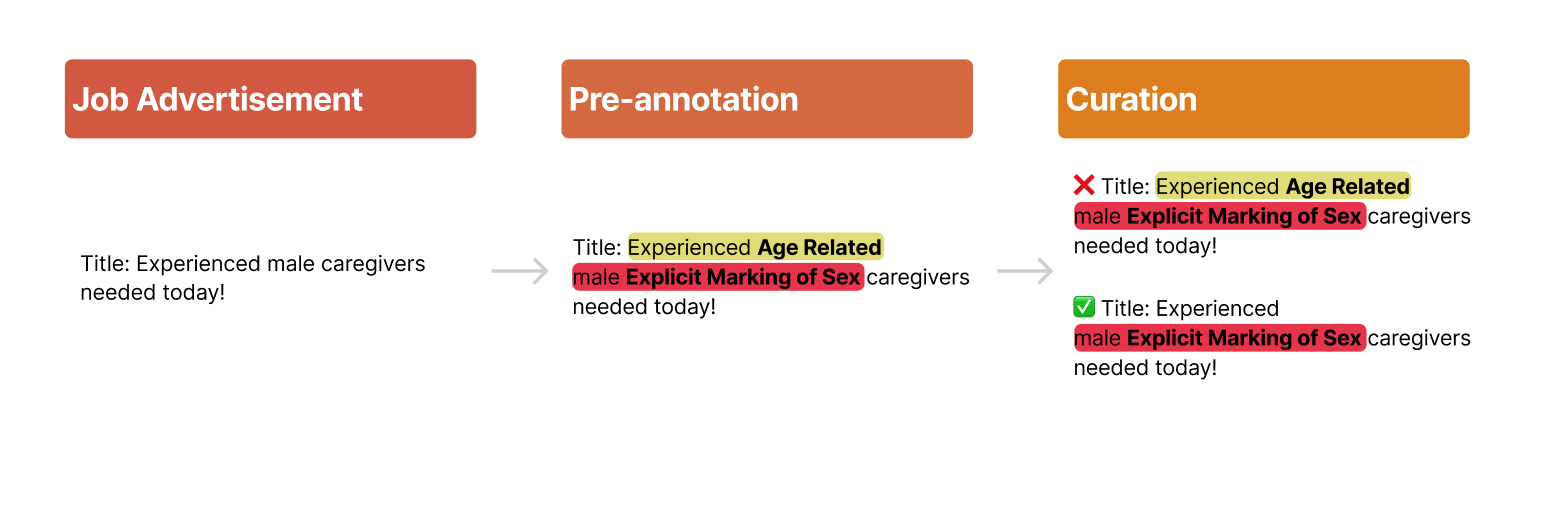
\includegraphics{images/annotation_process.png}

A key contribution expected from human annotators is the ability to discern bias based on context and appropriate spans. To facilitate this, annotators will receive complete job ads and be asked to examine specific sentences within each ad, allowing them to evaluate language in its full context.

The items to be annotated will consist of individual words or contiguous word spans extracted from real job advertisements. These advertisements originate from a diverse dataset encompassing multiple countries and industries.

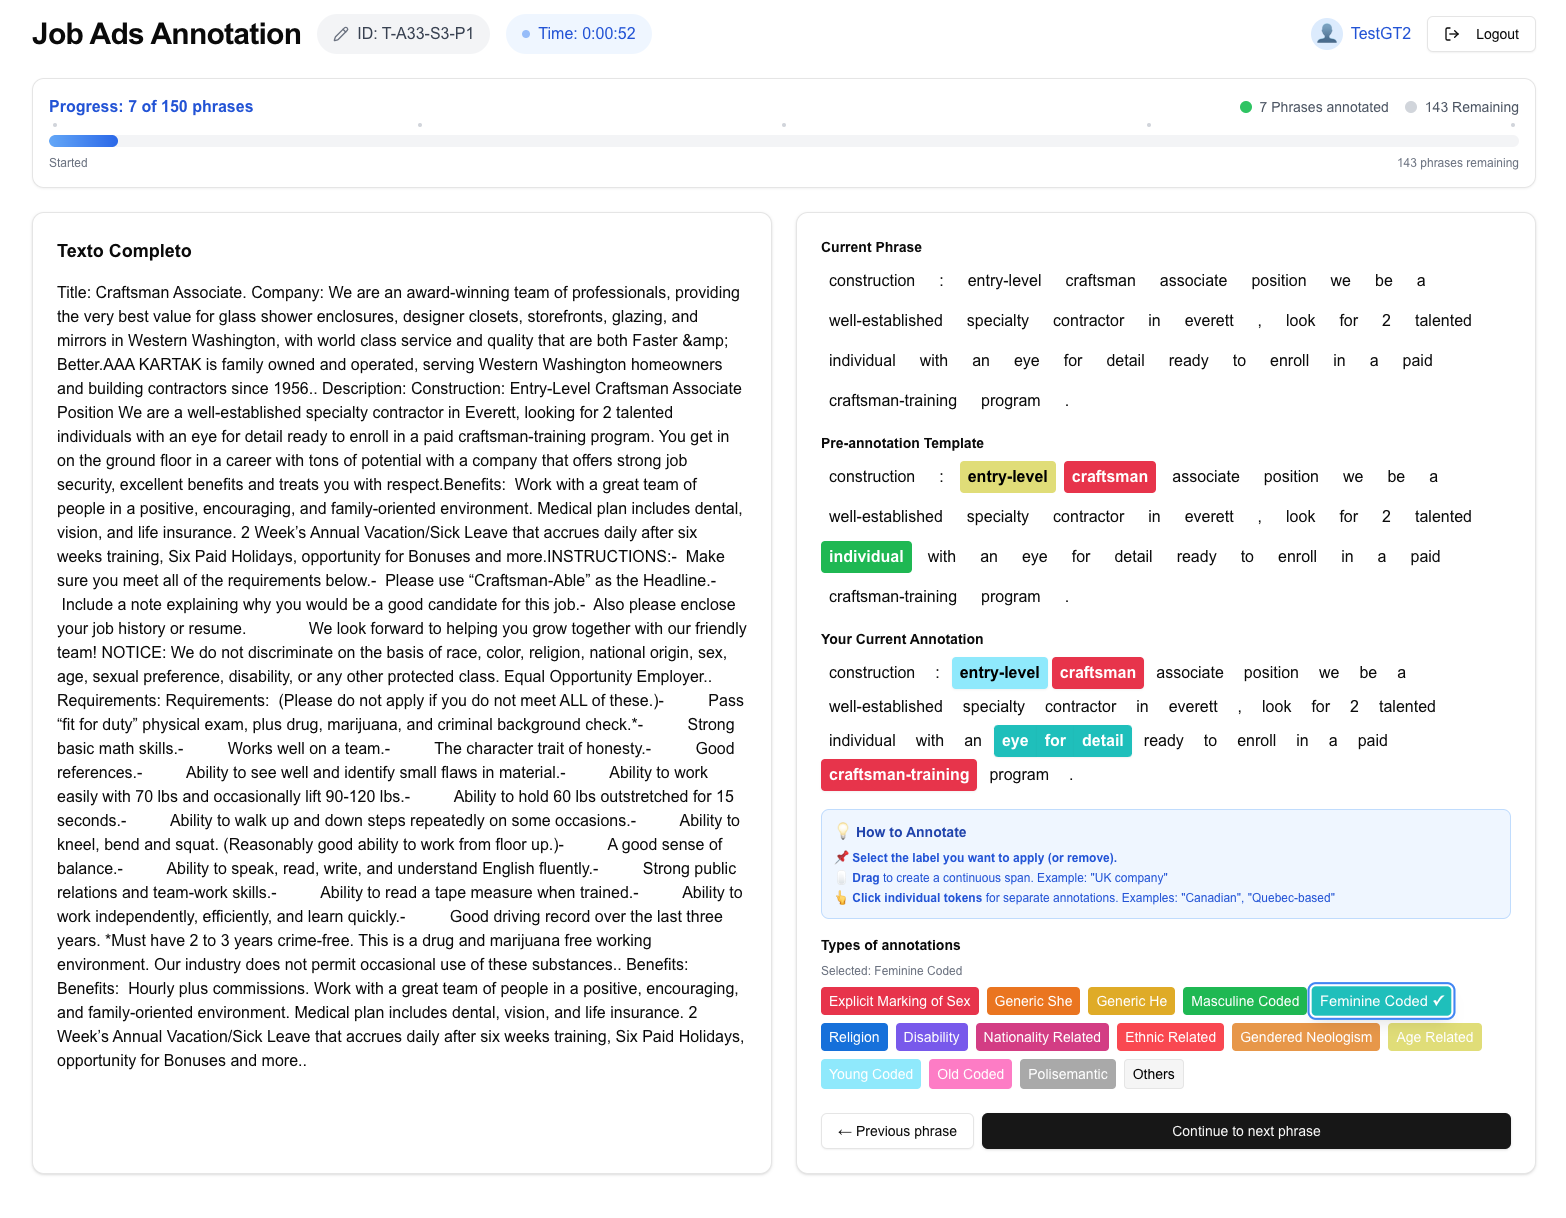
\includegraphics{images/annotation_app.png}

In this work, \textbf{bias is conceptualized as any language choice in a job advertisement that affects its perception by individuals or groups}, depending on their protected attributes. Such biases can either enhance or diminish the appeal or sense of belonging for the individual or group to a certain job. Other researchers address the idea that language-based biases can occur without overt or intentional discrimination, while some bias might discourage certain groups but not necessarily translate directly into illegal or explicit discriminatory practices (Heilman, 2012; Gaucher et al., 2011). Therefore, \textbf{bias in this context can be unconscious and does not always imply discrimination}, as their effect varies depending on the recipient and the specific circumstances of the bias.

\chapter{Summary}\label{summary}

\textbf{Task description}: Annotators will review individual sentences drawn from real job advertisements, with each full ad available for context. For every sentence, they must identify and highlight any words or phrases that exhibit bias.

\textbf{Labels}

\begin{itemize}
\item
  Age Bias:
  \textbf{\hyperref[age-explicit-bias]{{Age Related}}},
  \textbf{\hyperref[age-implicit-bias]{{Young Coded}}},
  \textbf{\hyperref[age-implicit-bias]{{Old Coded}}}.
\item
  Ethnicity Bias:
  \textbf{\hyperref[ethnicity-bias]{{Nationality Related}}},
  \textbf{\hyperref[ethnicity-bias]{{Ethnic Related}}}.
\item
  Gender Bias:
  \textbf{\hyperref[gender-exclusionary-terms]{{Explicit Marking of Sex}}},
  \textbf{\hyperref[gender-exclusionary-terms]{{Gendered Neologism}}},
  \textbf{\hyperref[generic-pronouns]{{Generic He}}},
  \textbf{\hyperref[generic-pronouns]{{Generic She}}},
  \textbf{\hyperref[gender-stereotypical-terms]{{Masculine Coded}}},
  \textbf{\hyperref[gender-stereotypical-terms]{{Feminine Coded}}}.
\item
  Religion Bias:
  \textbf{\hyperref[religion-bias]{{Religion Related}}}.
\item
  Disability Bias:
  \textbf{\hyperref[disability-bias]{{Disability Related}}}.
\item
  \textbf{\hyperref[polisemantic]{{Polisemantic}}}
\item
  \textbf{\hyperref[others]{{Others}}}
\end{itemize}

\textbf{Considerations}

\begin{itemize}
\item
  The bias categories are designed to be mutually exclusive and should not overlap.
\item
  As a general rule, annotators should highlight the longest continuous phrase that conveys the bias. For example, in the sentence ``accommodation can be made for physical disability,'' mark ``physical disability'' rather than just ``disability.''
\item
  Please note that there is a dedicated category for polysemous terms---see the Polisemantic Class section for details \hyperref[polisemantic]{here}.
\item
  Annotators should take care when tagging biased language that appears in close proximity. In other words, if a sentence contains two words of the same bias category and each word qualifies on its own---each must be annotated separately.
\end{itemize}

\chapter{Type of Biases}\label{type-of-biases}

In this section there is the definition of every type of bias of this research.

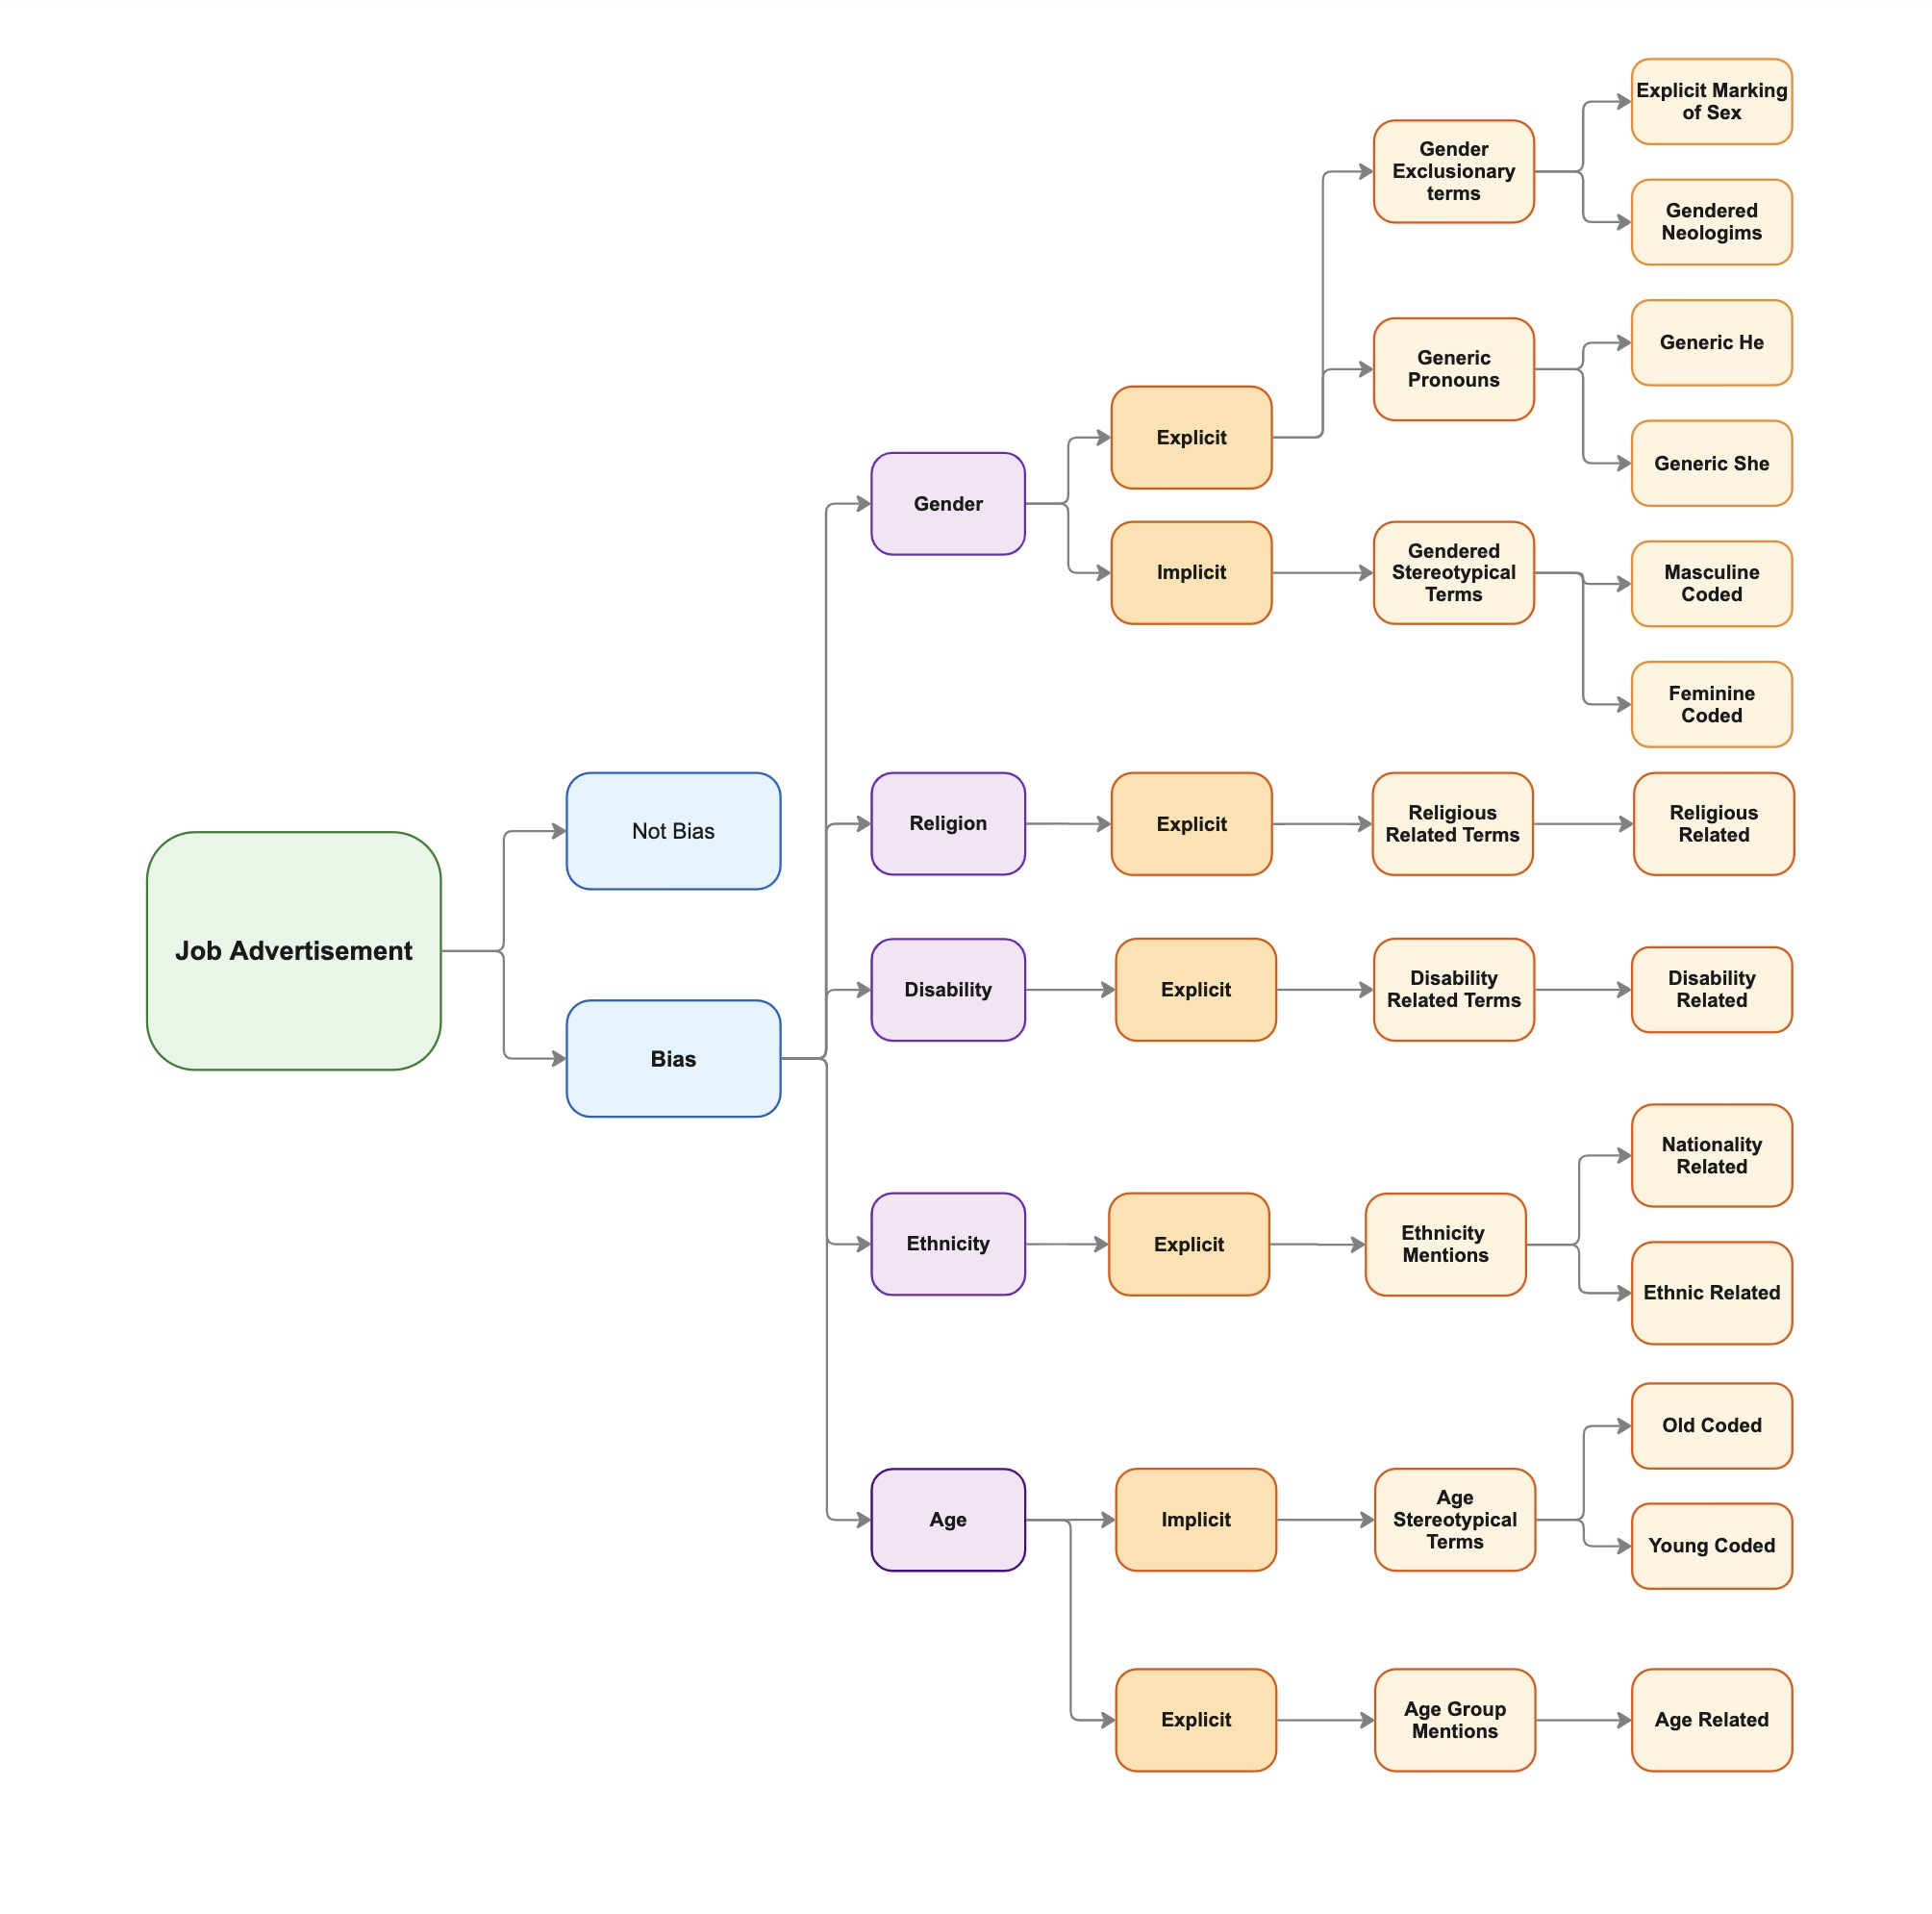
\includegraphics{images/Taxonomy-v9.jpg}

\section{Explicit Age Bias}\label{explicit-age-bias}

\subsection*{Age Mentions}\label{age-explicit-bias}
\addcontentsline{toc}{subsection}{Age Mentions}

This category includes any direct or indirect reference to an applicant's age group in a job advertisement. Whether it's a clear requirement or a more subtle allusion, these mentions influence how candidates perceive their eligibility. Although specifying experience is often necessary, we mark every term or phrase that conditions applicant selection by age as explicit bias.

{\textbf{Age Related}}

In job advertisements, references to age can take many forms---ranging from explicit age requirements to subtle age cues woven into the job title or description.

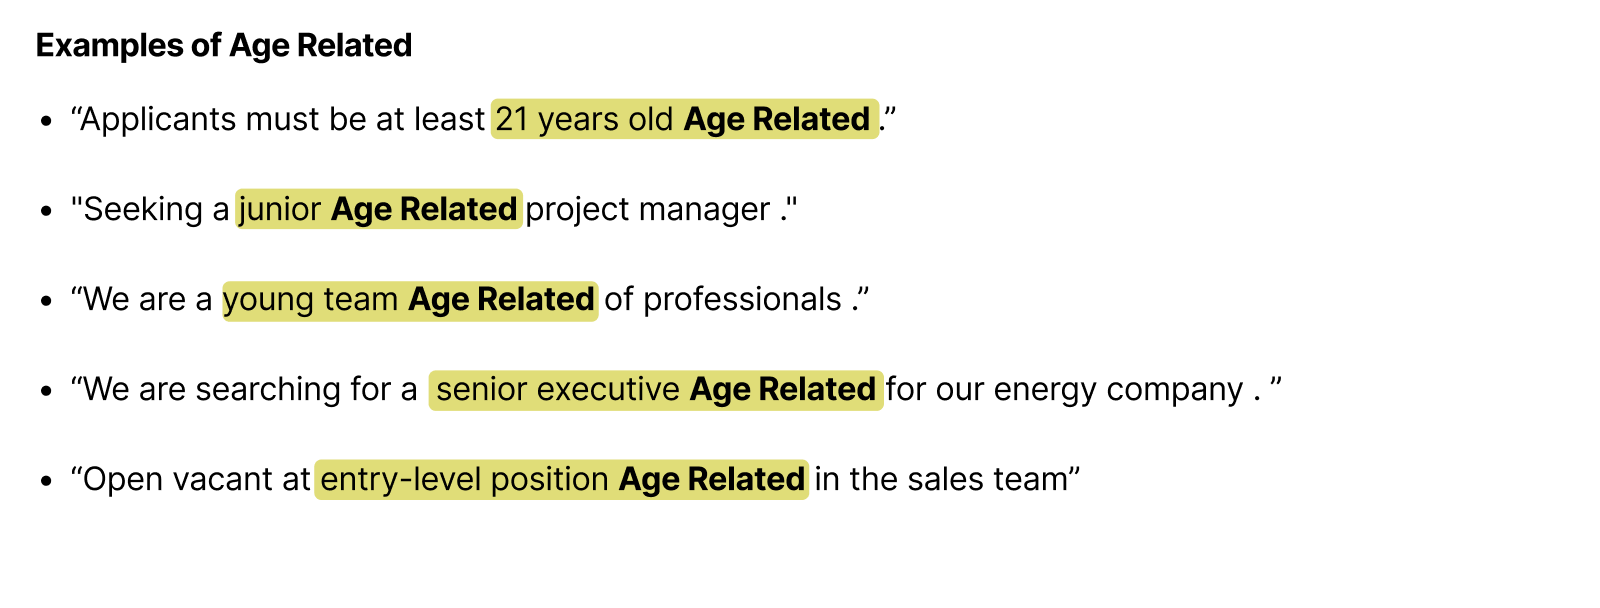
\includegraphics{images/Age_Related.png}

\section{Implicit Age Bias}\label{implicit-age-bias}

\subsection*{Age Stereotypical Terms}\label{age-implicit-bias}
\addcontentsline{toc}{subsection}{Age Stereotypical Terms}

This bias consists of any phrasing that relies on age stereotypes---such as endorsements of ``digital natives'' or appeals to ``experienced professionals.'' It can be woven into any part of the ad, from the company profile to linguistic choices in the benefits. Since it operates subtly through semantic nuance, it qualifies as implicit age bias. This is an implicit form of age bias, driven by meaning and context rather than clear-cut rules. We further subdivide this class into Young-Coded and Old-Coded language.

{\textbf{Young Coded}}

This category covers any linguistic choice in a job ad that specifically appeals to a younger audience. These cues aren't meant to exclude older applicants; they simply aim to attract younger talent.

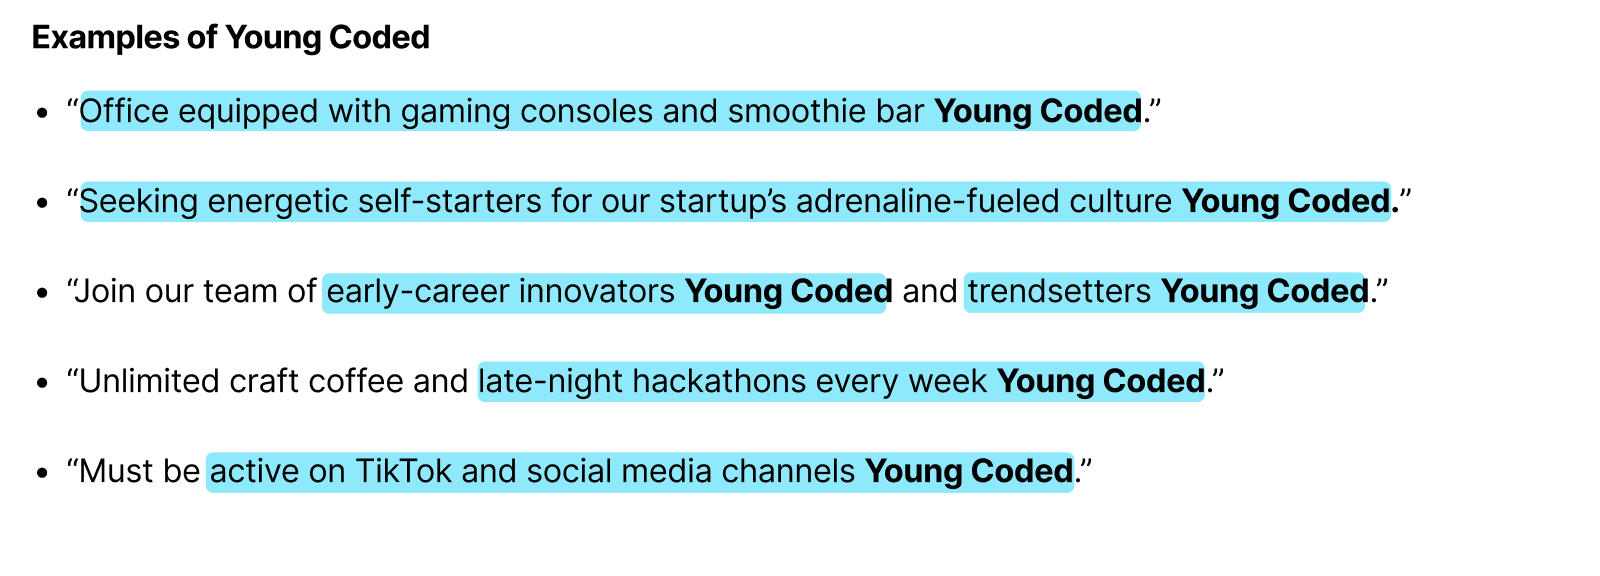
\includegraphics{images/example_young_coded.png}

{\textbf{Old Coded}}

This category encompasses phrases or wording that signal a preference for more mature candidates. Like Young-Coded terms, these expressions are designed to draw in a specific age group rather than to push others away. Be careful not to conflate general formality with Old-Coded bias (e.g., ``decades of experience'' vs.~everyday professional tone).

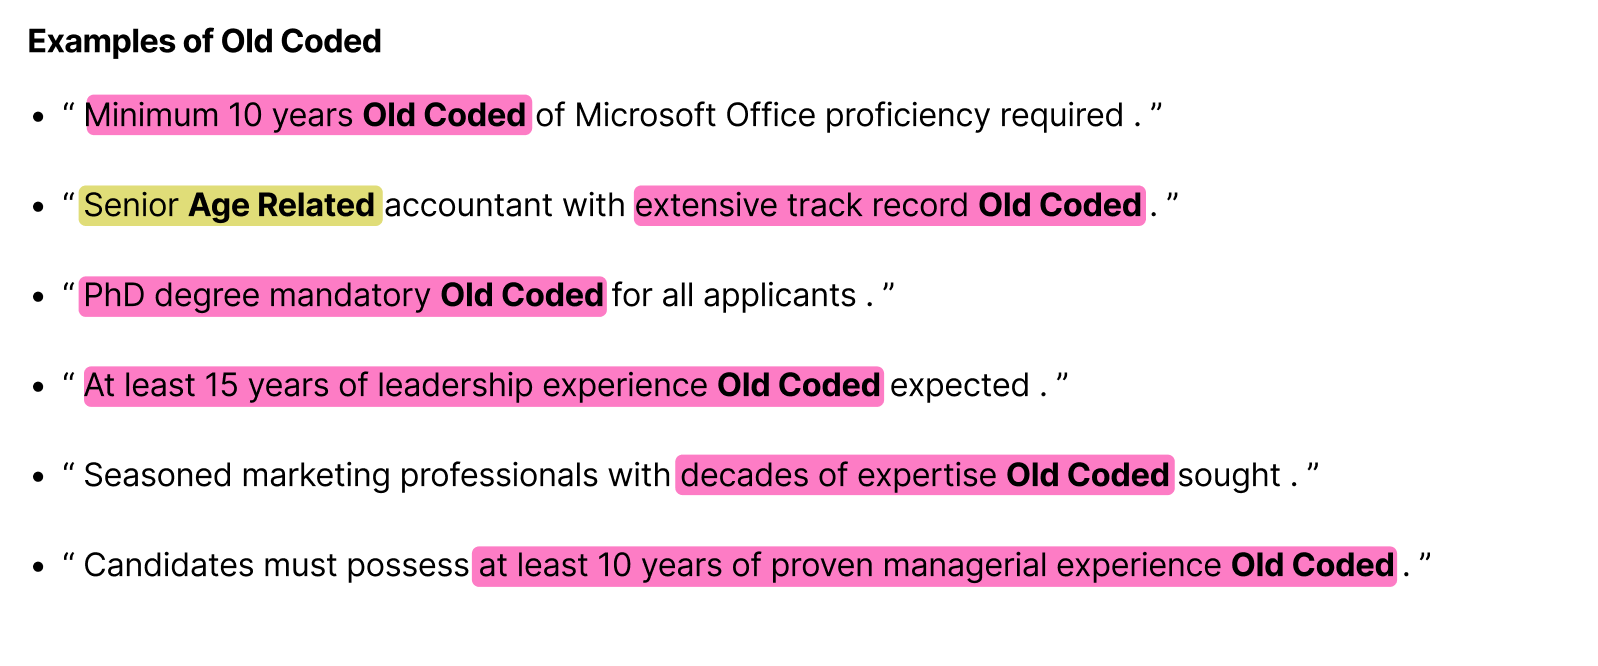
\includegraphics{images/Old_Coded.png}

\section{Explicit Ethnicity Bias}\label{explicit-ethnicity-bias}

\subsection*{Ethnicity Mentions}\label{ethnicity-bias}
\addcontentsline{toc}{subsection}{Ethnicity Mentions}

This category covers any unambiguous mention of ethnicity in a job posting, whether in the company name, candidate requirements, or descriptive phrases. Such explicit ethnic references---like insisting on a specific nationality or calling out a particular heritage---can significantly influence who applies, so we define them as biased. While many attributes can signal ethnicity, this study focuses on two main types: nationality and other ethnic related terms. Keep in mind that any religious references should be classified under Explicit Religion Bias rather than here.

{\textbf{Nationality Related}}

Within the broader category of ethnic biases, we spotlight nationality bias because it frequently appears in job ads. Nationality bias includes any explicit reference to a specific nation, nationality, city, state, or province. However, references to continents or clusters of countries are excluded. Mentions of language are also not necessarily treated as nationality bias; their classification depends entirely on how they're used.

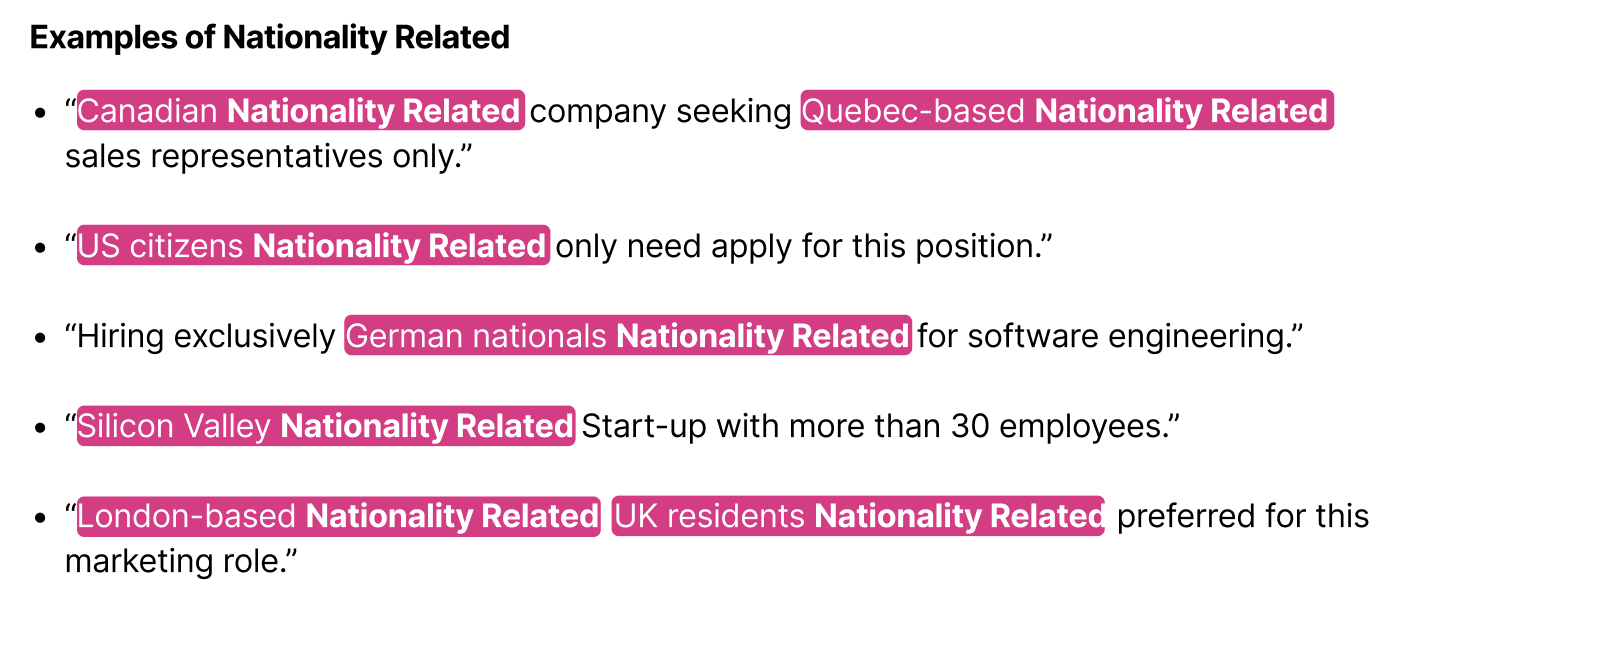
\includegraphics{images/Nationality-Related.png}

{\textbf{Ethnic Related}}

Any term or expression that evokes ethnic characteristics---consciously or unconsciously---apart from nationality. Examples include references to racial group, complexion, region of ancestral origin, or cultural lineage.

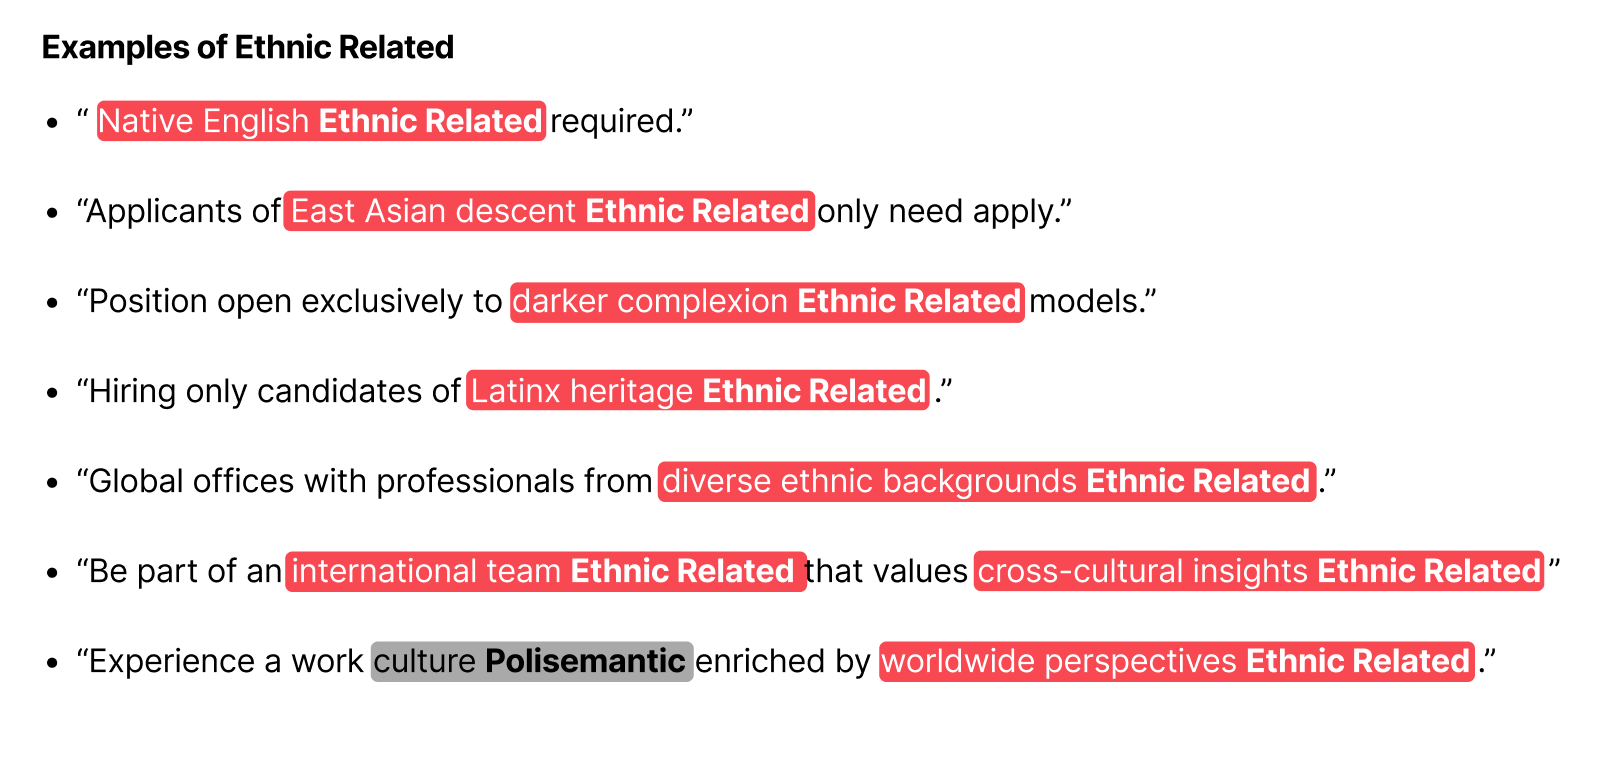
\includegraphics{images/Ethnic-Related.png}

\section{Explicit Gender Bias}\label{gender-bias}

\subsection*{Gender Exclusionary Terms}\label{gender-exclusionary-terms}
\addcontentsline{toc}{subsection}{Gender Exclusionary Terms}

Exclusionary terms occur when a gender-neutral entity is described using gender-exclusive language. For instance, adding a gender-specific sub-word (e.g., ``man'') to a gender-neutral occupational term (e.g., ``police'') results in ``policeman.'' This construction implies that all police officers are men, thereby excluding women. Conversely, appending ``woman'' to ``police'' to form ``policewoman'' suggests that all police officers are women. The use of exclusionary terms has been shown to carry negative societal implications. Sex-biased wording can affect perceptions of a career's attractiveness (Briere and Lanktree, 1983), and languages with gendered occupational terms have been associated with disproportionate labor force participation (Gay et al., 2013).

{\textbf{Explicit Marking of Sex}}

The use of explicit sex demarcations in job advertisements constitutes a form of Gender-Exclusive Occupational Terms bias. This category covers instances where an inherently gender-neutral role or occupation is described using a word that unambiguously denotes one gender. Such markings often appear at the word level and clearly signal a specific gender.

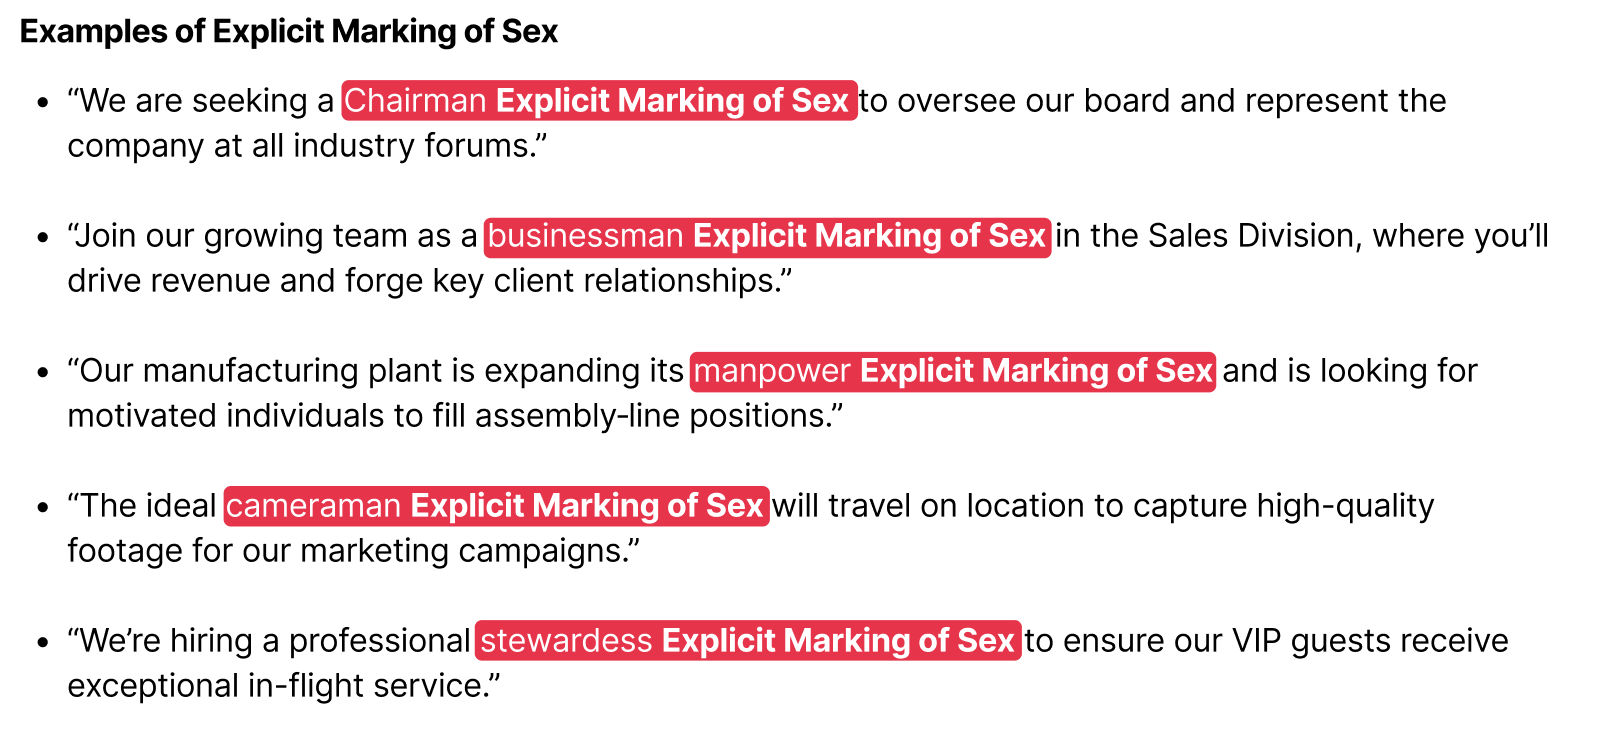
\includegraphics{images/Explicit-Marking.png}

{\textbf{Gendered Neologism}}

Gendered Neologisms are newly coined, gender-specific terms that are emerging into mainstream usage. Although they share similarities with explicit marking of sex in that they exclude one gender, they differ by virtue of their novelty and evolving acceptance in everyday language. This type of bias is annotated at the word level, as it involves the creation of new exclusionary terms.

Examples: Man-bread, Man-sip, Man-bun, Girlboss, SheEO

\subsection*{Generic Pronouns}\label{generic-pronouns}
\addcontentsline{toc}{subsection}{Generic Pronouns}

Pronouns typically correspond to the gender of their referents. However, when the referent is sex-indefinite, the pronoun is used in a generic sense, effectively generalizing gender onto a neutral subject. The most notable form of a generic pronoun sentence occurs when a pronoun's referent is a sex-indefinite occupation. When a pronoun refers to an occupation rather than a sex-definite person (subject), it becomes generic.

{\textbf{Generic He}}

Generic He refers to instances where a sex-indefinite role or description is associated with a male pronoun. This use often reflects implicit gender bias by defaulting to a male reference when the subject's gender is not specified. Due to its dependence on context, this bias is assessed at the sentence level.

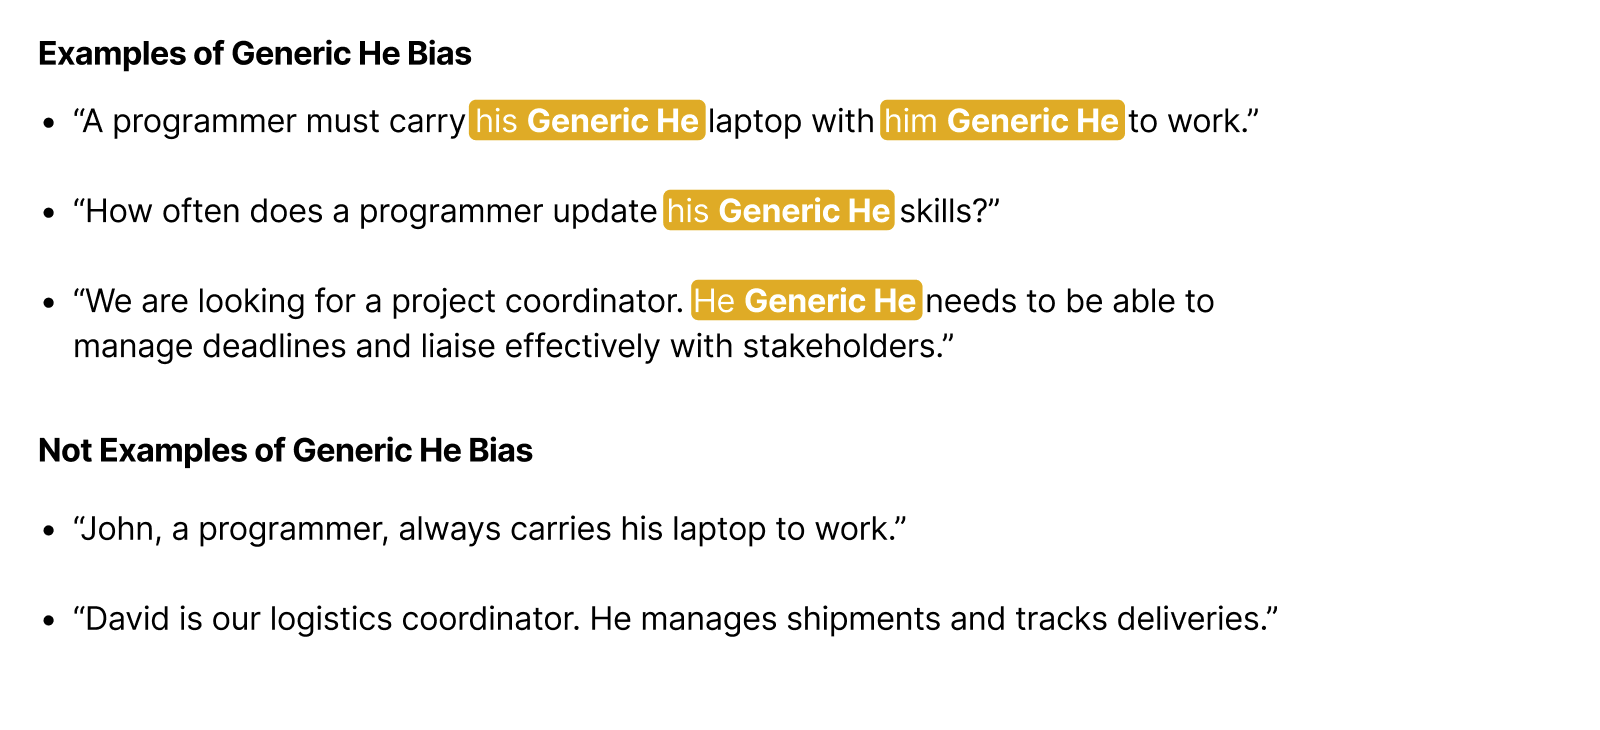
\includegraphics{images/Generic-He.png}

{\textbf{Generic She}}

Generic She denotes instances where a sex-indefinite role or description is associated with a female pronoun. This usage may introduce bias by implying that a particular role should be associated with a female perspective when the role itself is gender-neutral. Like Generic He, this bias is evaluated within the context of the sentence.

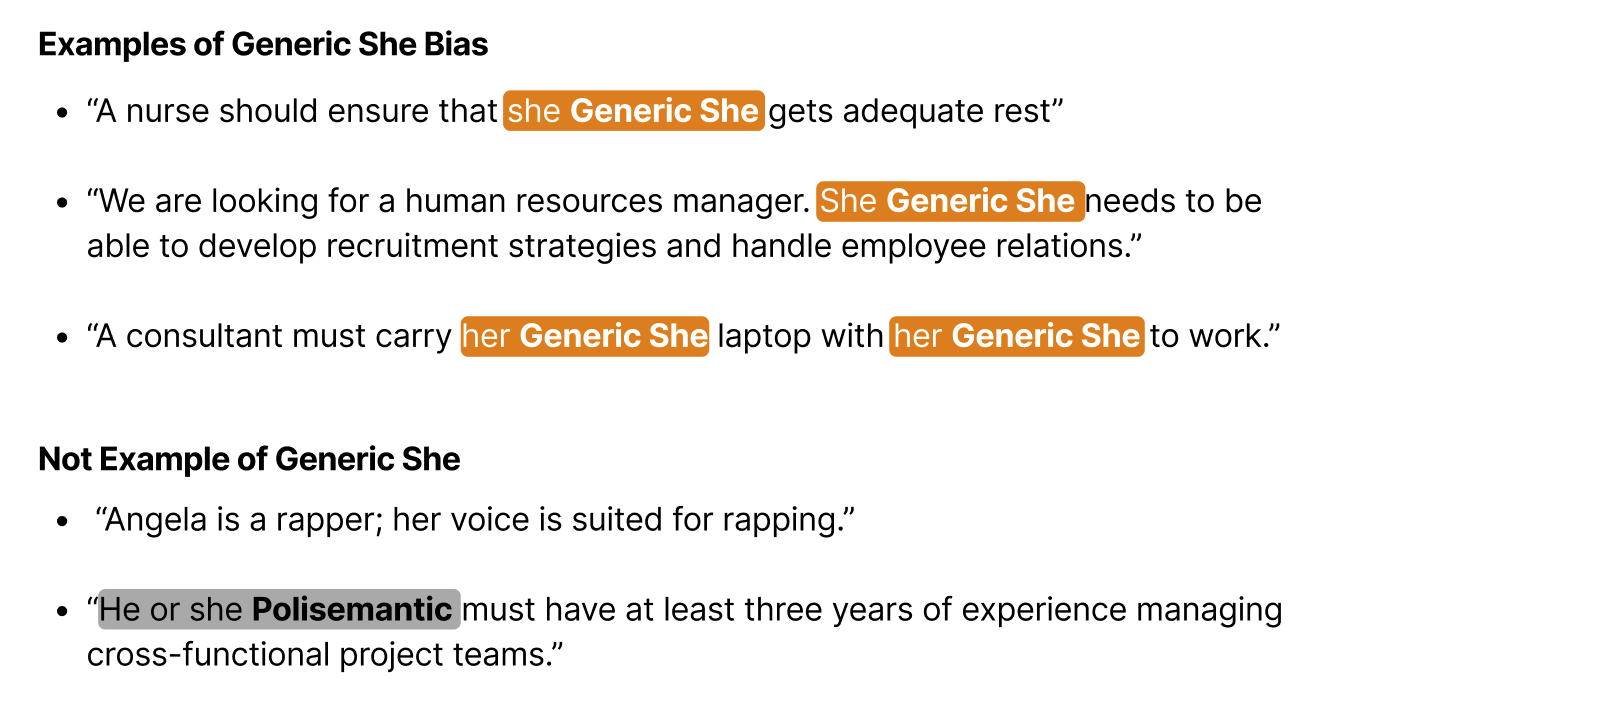
\includegraphics{images/Generic-She.png}

\section{Implicit Gender Bias}\label{implicit-gender-bias}

Subtle language choices that suggest a preference for one gender without explicitly naming it. In this instance we will be working mainly with words or sentences that have a strong stereotype associated with a gender in the context of work recruitment.

\subsection*{Gendered Stereotypical Terms}\label{gender-stereotypical-terms}
\addcontentsline{toc}{subsection}{Gendered Stereotypical Terms}

This category covers the inclusion of words or short phrases in job advertisements that carry gender stereotypes. Studies demonstrate that such wording can affect applicants' attitudes and choices depending on their gender (Gaucher et al, 2011). Since job ads use a formal style, these subtle signals are considered implicit bias.

{\textbf{Feminine Coded}}

This type of bias refers to the use of words or language choices associated with female stereotypes, speccially those related to work enviroment. Some adjectives and subtle signs can influence in the pool of candidates of the job offer.

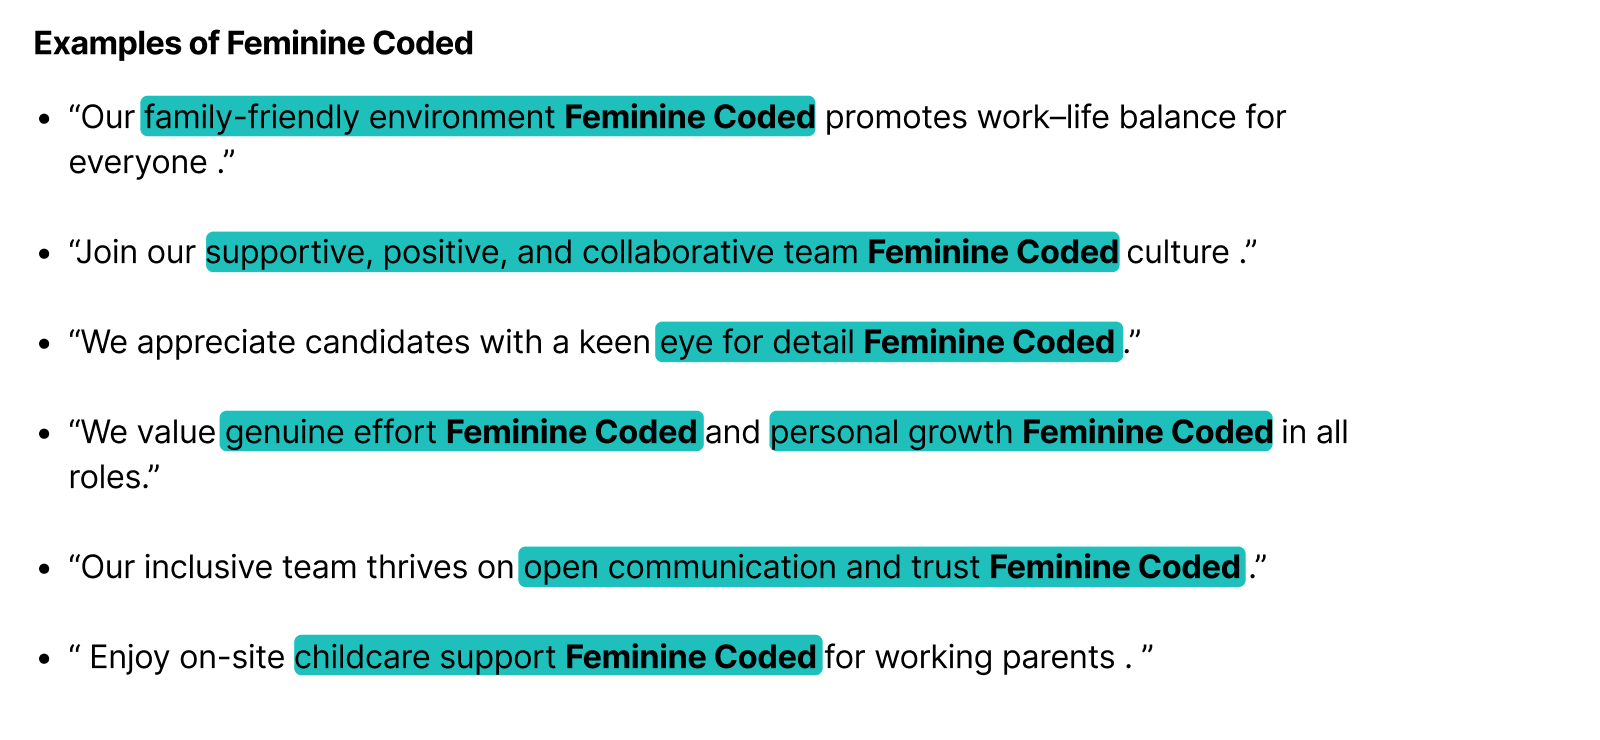
\includegraphics{images/Feminine-Coded.png}

{\textbf{Masculine Coded}}

Use of words associated with male stereotypes (e.g., ``aggressive'', ``dominant'') that subtly signal a male-oriented role or culture.

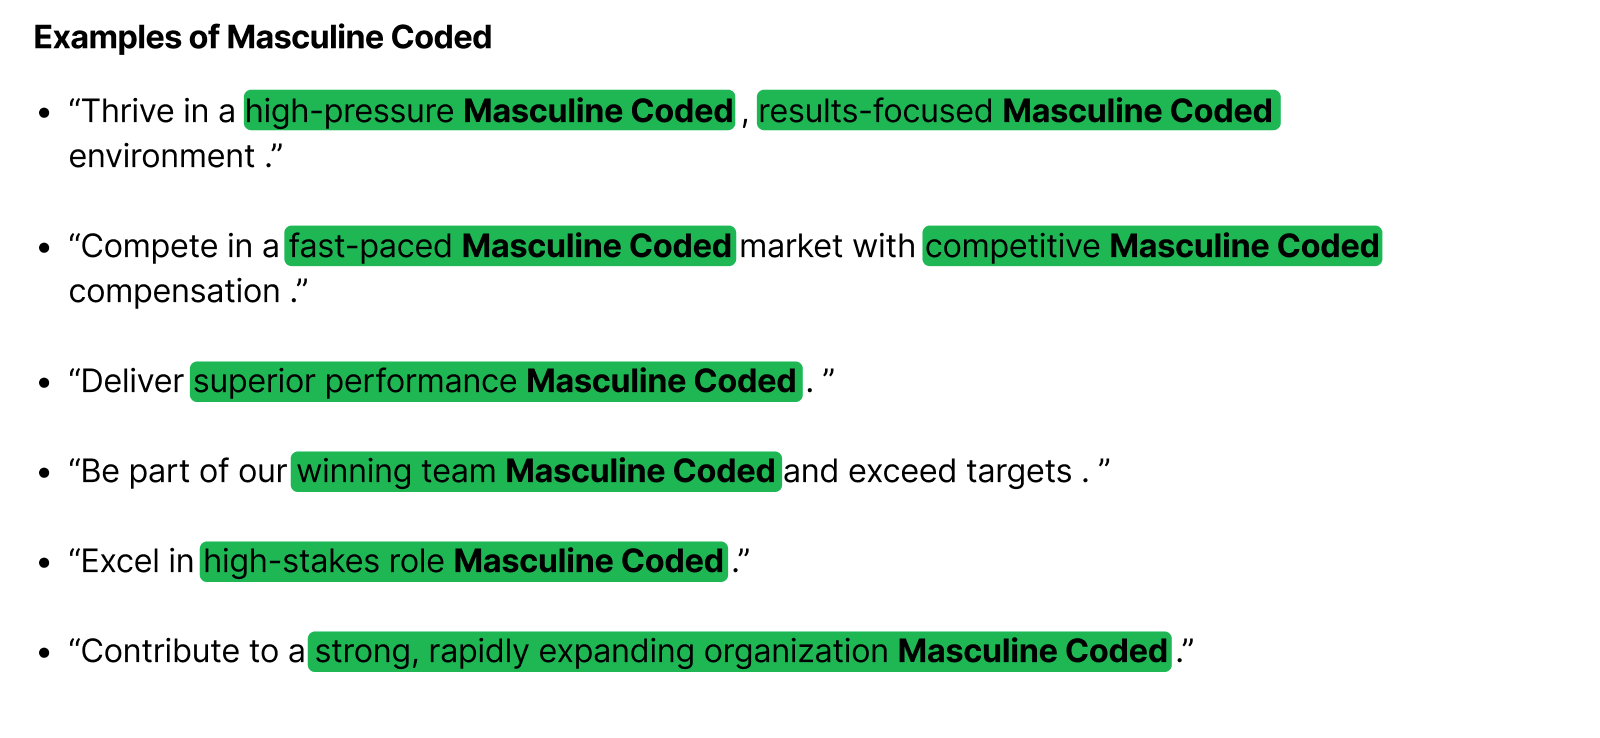
\includegraphics{images/Masculine-Coded.png}

\section{Explicit Religion Bias}\label{explicit-religion-bias}

\subsection*{Religious Related Terms}\label{religion-bias}
\addcontentsline{toc}{subsection}{Religious Related Terms}

Mentions of terms or groups directly and explicitly tied to a religion constitute a bias category in job advertisements, framing the text within a particular religious worldview. Such explicit references can immediately influence potential candidates according to their own beliefs. Although some mentions may be subtle, we treat any reference to a religion or belief system as a single bias class in job postings.

{\textbf{Religion Related}}

Mentions of religion in job advertisements can take many forms---from explicit faith-based requirements to subtle nods toward religious institutions. Regardless of how overt or understated they may be, any word or phrase that references a religion, belief system, or religious organization belongs in this category.

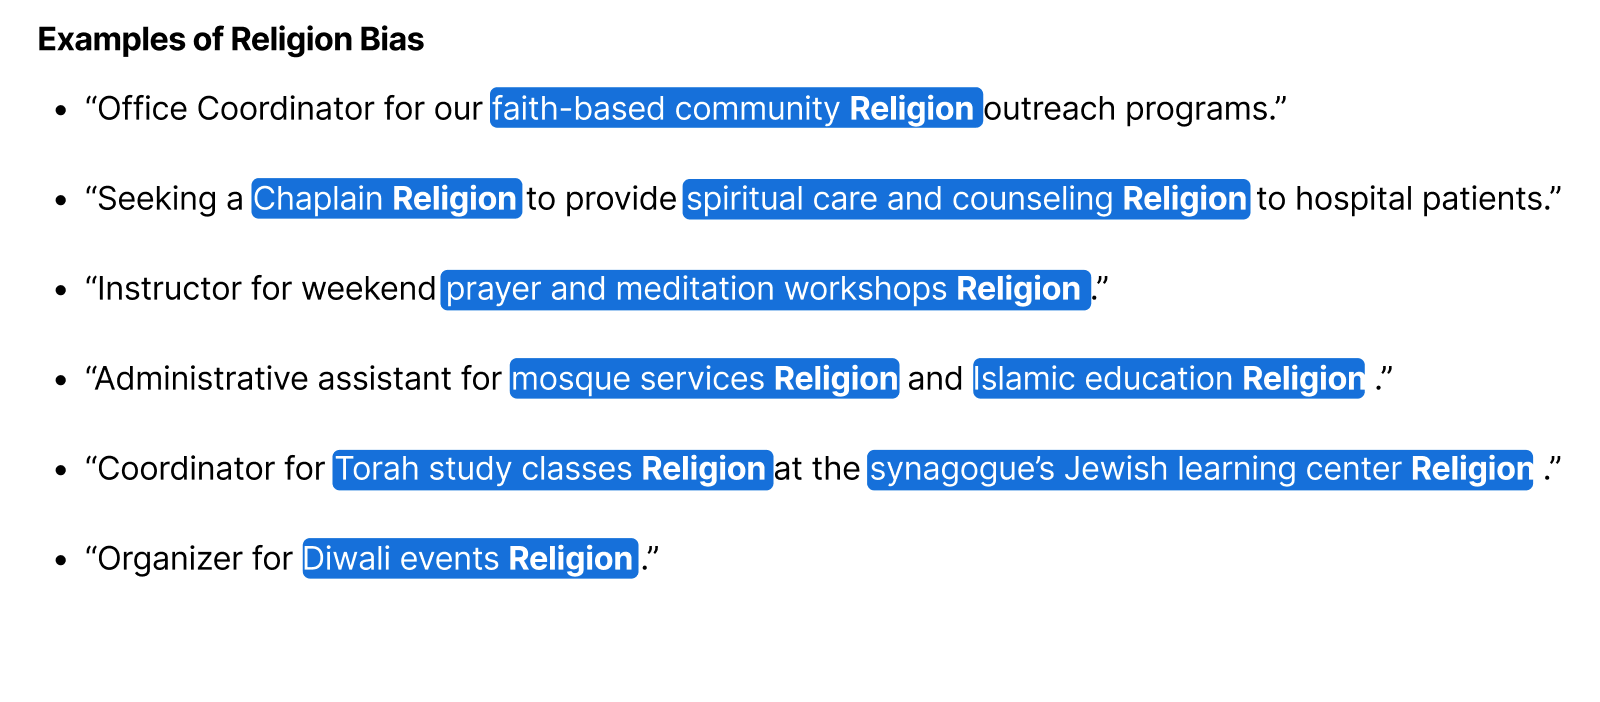
\includegraphics{images/Religion-Related.png}

\section{Explicit Disability Bias}\label{explicit-disability-bias}

\subsection*{Disability Related Terms}\label{disability-bias}
\addcontentsline{toc}{subsection}{Disability Related Terms}

This category covers any words or phrases in job advertisements that reference disability---whether it's explicit benefits (e.g., ``disability insurance'') or non-discrimination clauses for candidates with impairments. Although most of these statements are intended as positive accommodations, they still influence how applicants with disabilities perceive and respond to the opportunity. Therefore, any mention of disability in a job posting is treated as a single bias class, since it can alter candidates' behavior and expectations.

{\textbf{Disability Related}}

Terms reflecting disability bias might be as brief as the word ``disability'' or as elaborate as outlining specific conditions. You can find this bias in any section of a job ad.

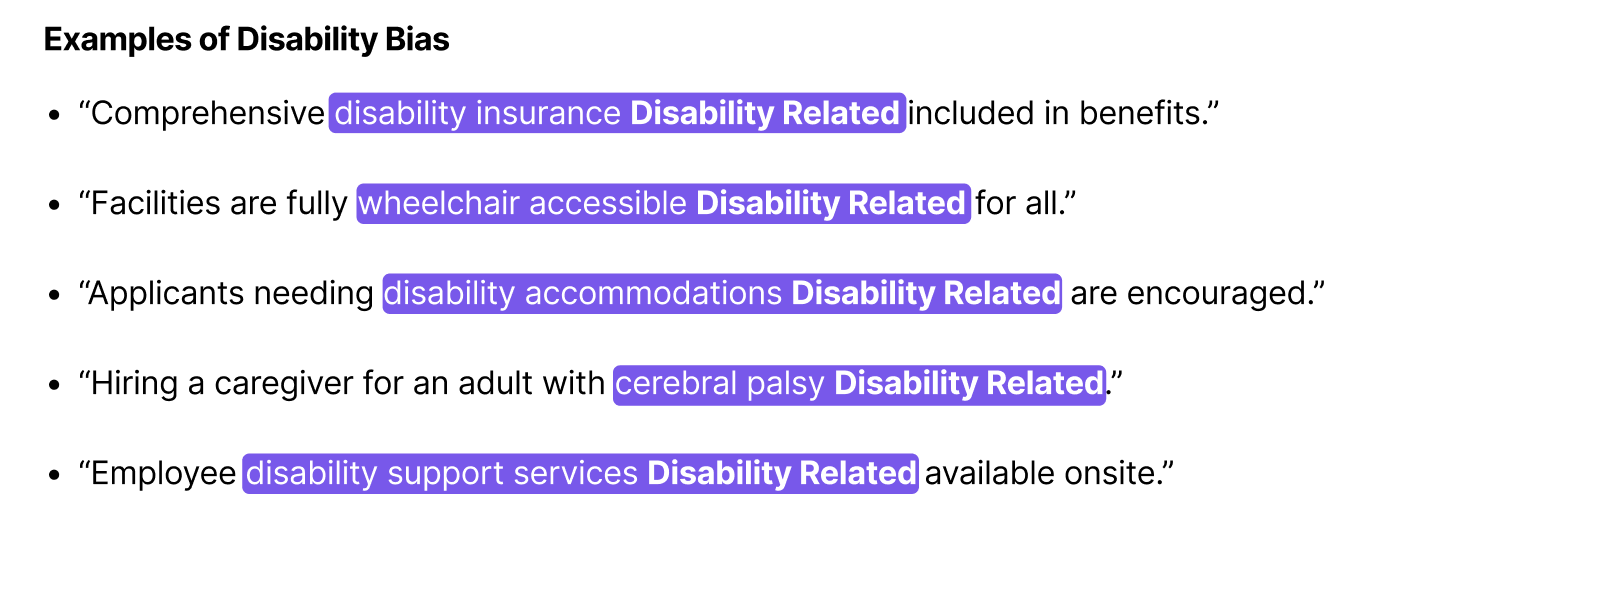
\includegraphics{images/Disability-Related.png}

\chapter{Polisemantic Class}\label{polisemantic}

\textbf{Context}

Job advertisements are typically written in a formal register, where many terms exhibit polysemy---that is, they carry multiple senses, some of which may imply bias in other contexts while remaining neutral here. Because lexicon-based detectors lack the contextual awareness to distinguish these senses, they often overlook words that are harmless in a job ad but problematic elsewhere.

\textbf{Definition}

We define the {\textbf{Polisemantic}} class as all words that function neutrally within a job advertisement yet could convey bias in a different setting. Annotators must flag every instance of such polysemous vocabulary---regardless of lexicon matches---and confirm its unbiased usage in context.

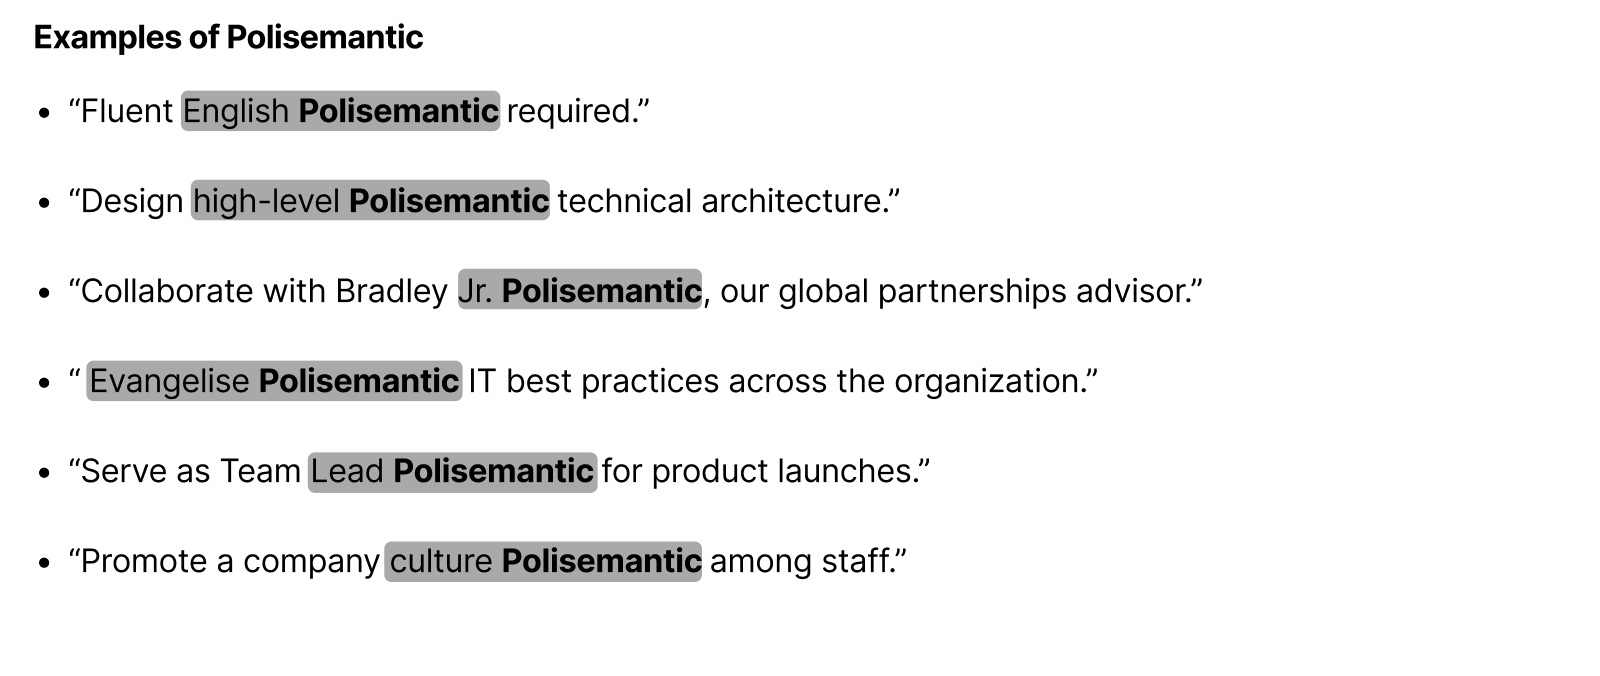
\includegraphics{images/Polisemantic.png}

\chapter{Others Class}\label{others}

\textbf{Context}

As part of this research, we carried out both theoretical and empirical analyses to uncover new types of bias in job advertisements. We recognize that additional or unexpected biases may surface---ones not addressed by the existing categories but appearing more frequently than anticipated. To accommodate these discoveries, we introduce a dedicated class that allows annotators to flag such cases for later review.

\textbf{Definition}

The Others class covers any bias or special case identified by annotators that does not fit within the predefined categories. This could include intersectional biases---when a term exhibits characteristics of more than one category (e.g.~a mention botth Masculine-Coded and Young-Coded). Other cases could be sexual orientation or socioeconomic status, and any novel bias instances spotted during annotation that merit further investigation.

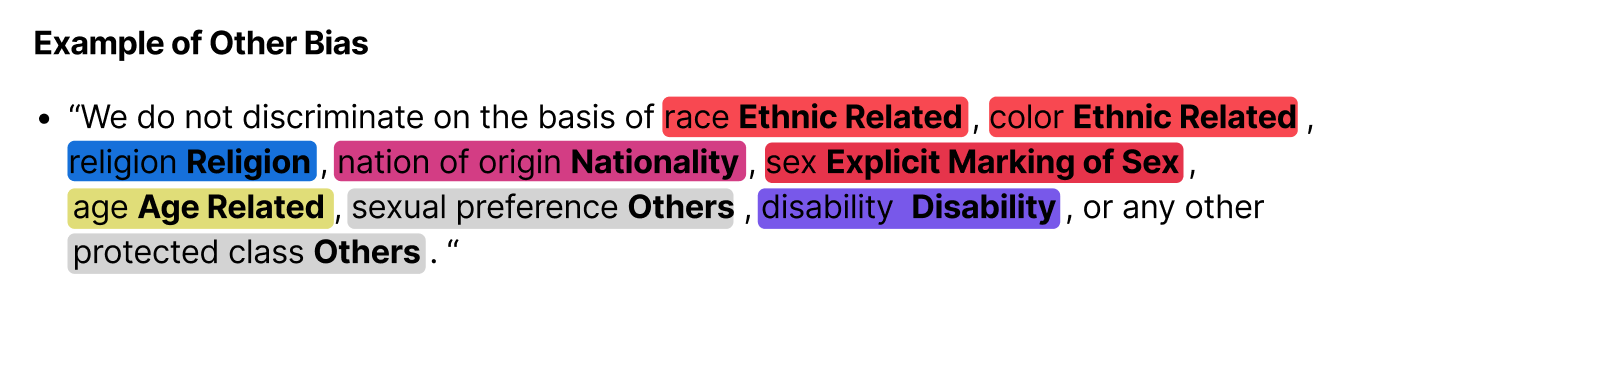
\includegraphics{images/Others.png}

\chapter{Examples}\label{examples}

List of examples of every class and how they should be annotated.

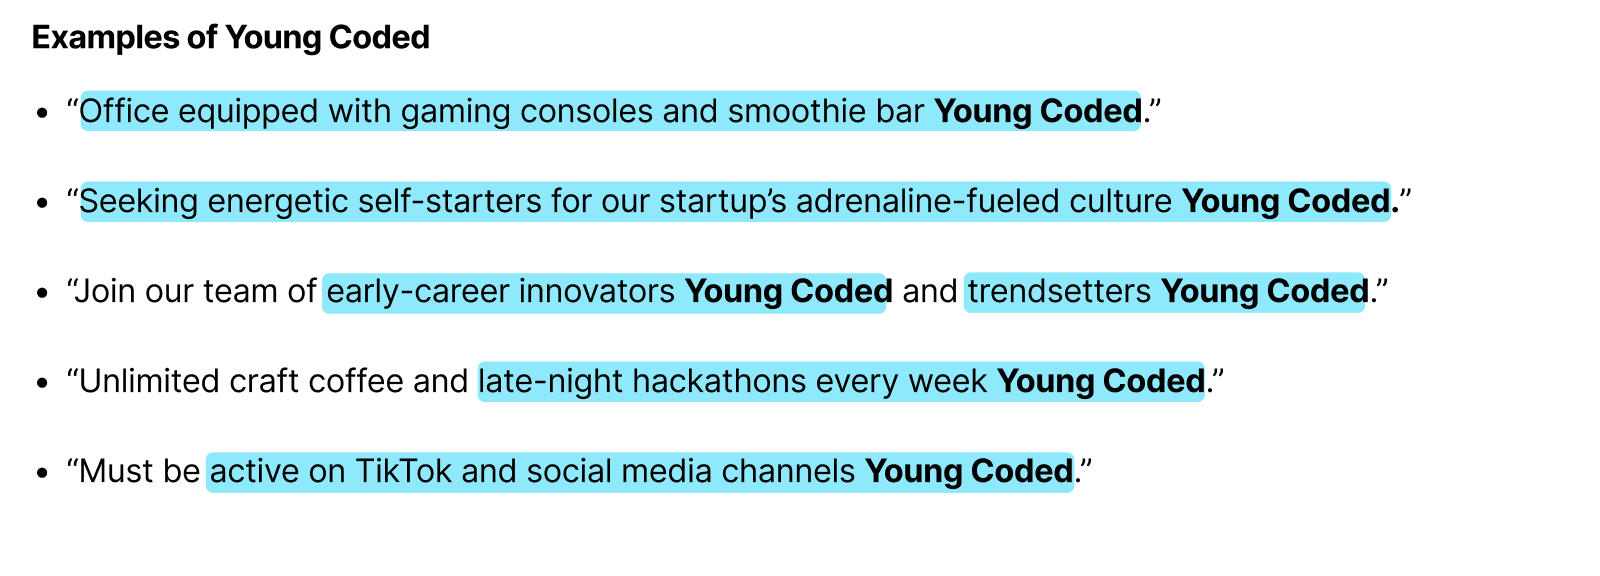
\includegraphics{images/example_young_coded.png}
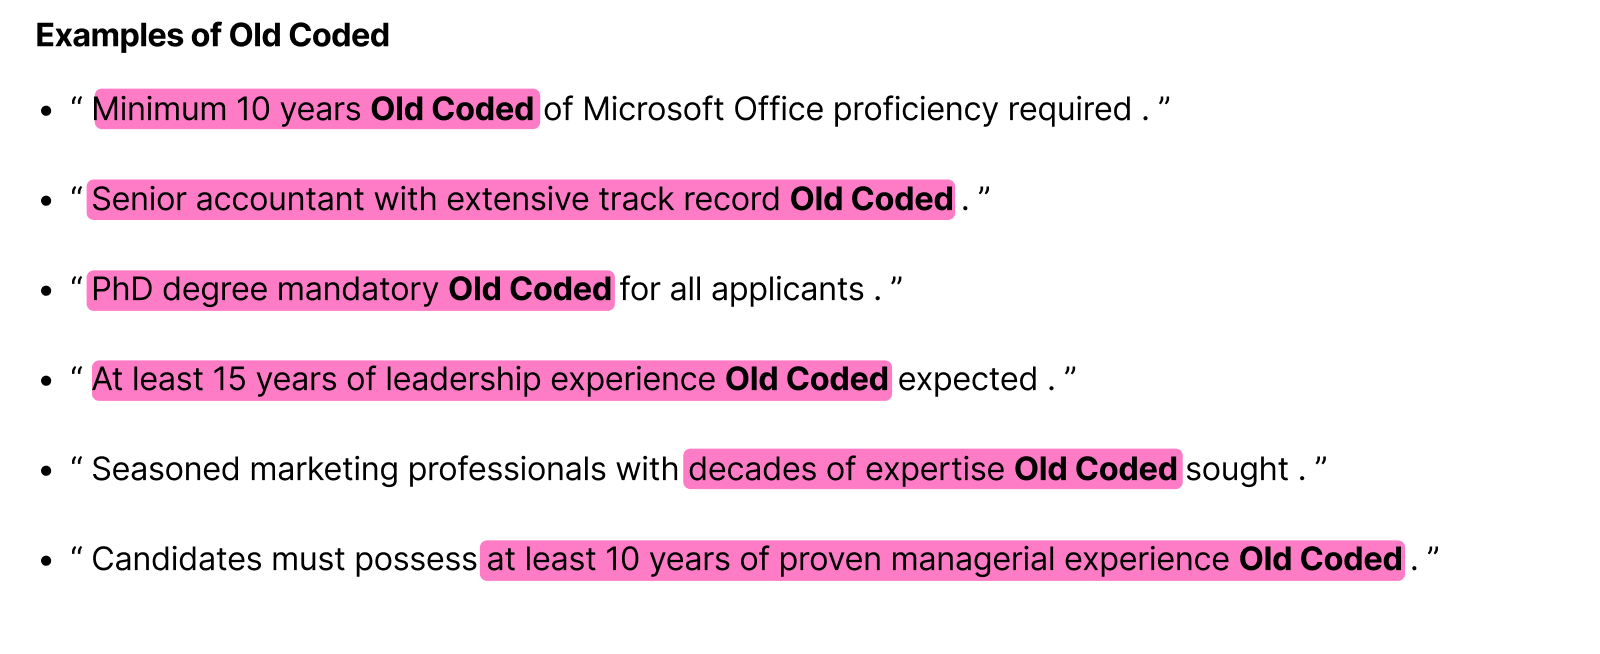
\includegraphics{images/Old-Coded.png}
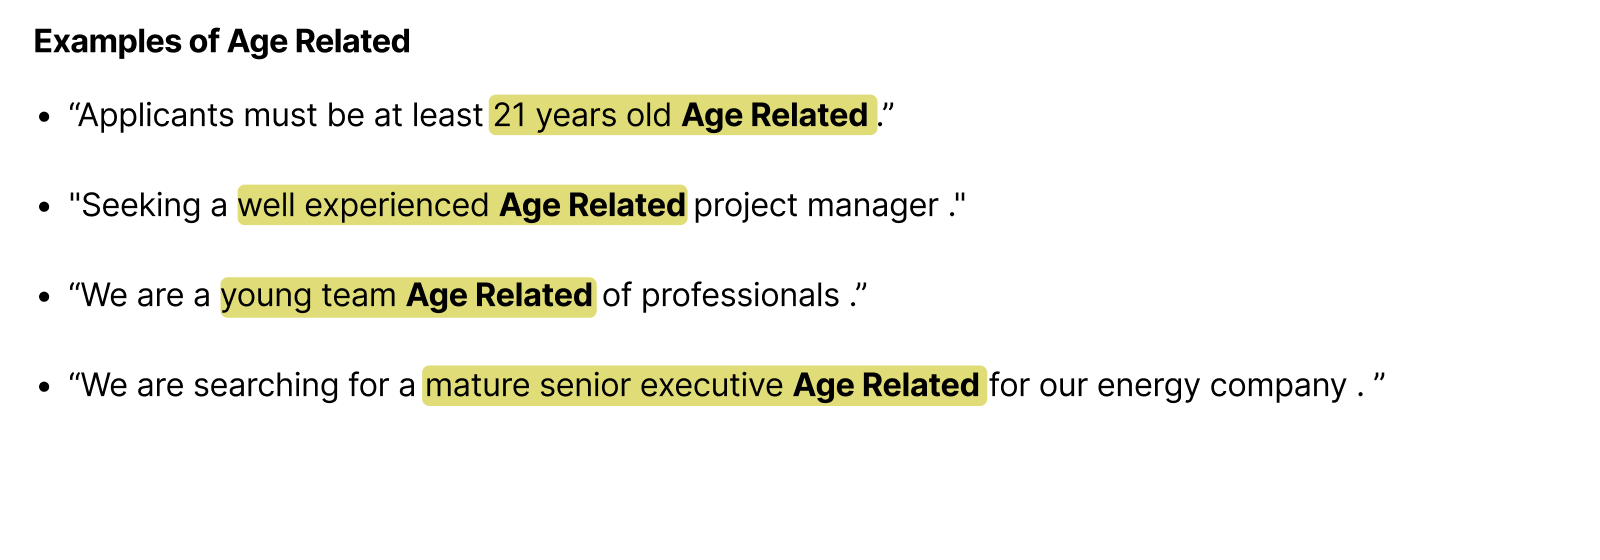
\includegraphics{images/Age-Related.png}
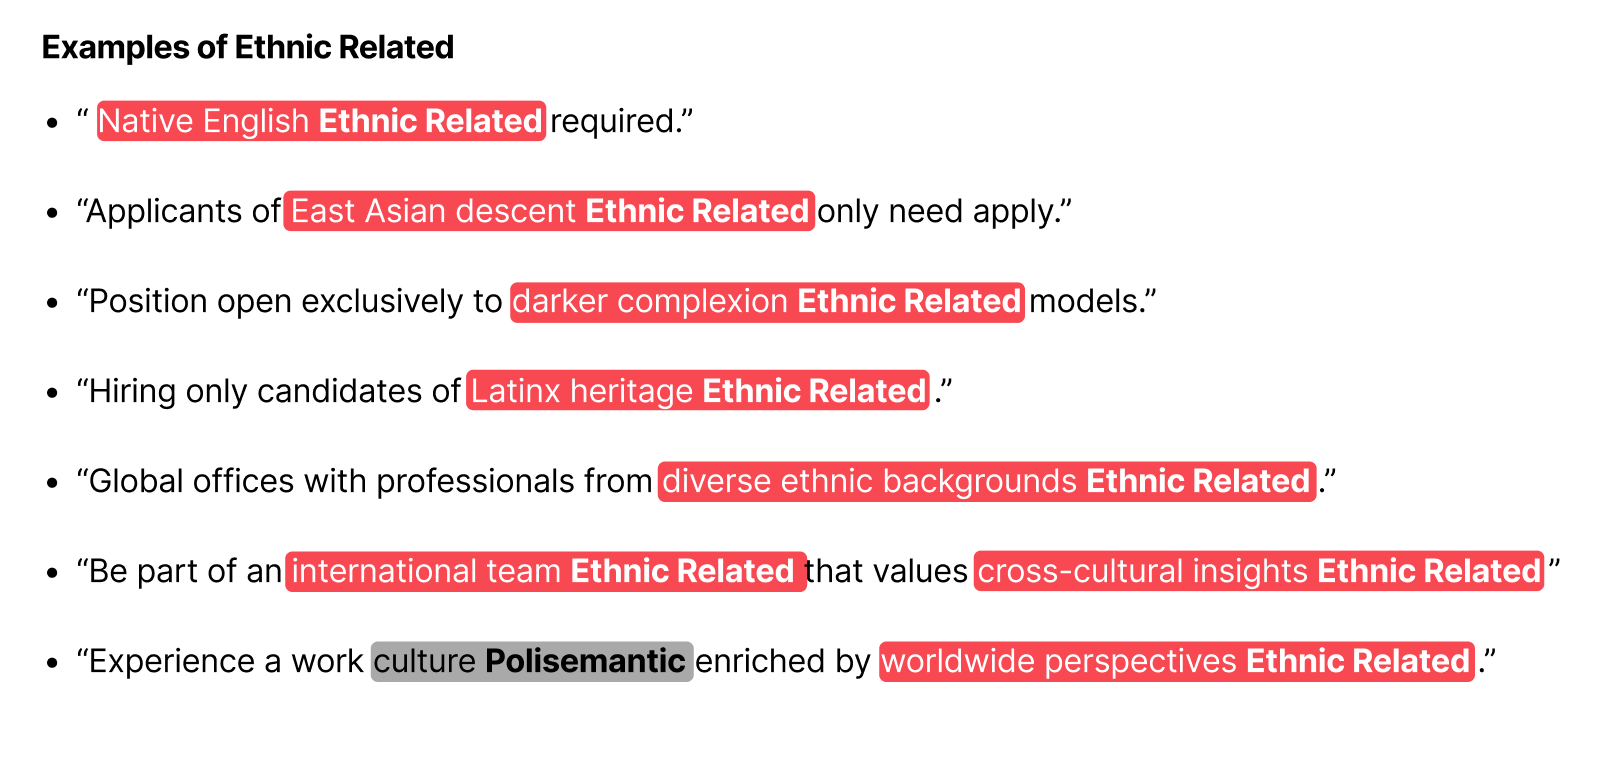
\includegraphics{images/Ethnic-Related.png}
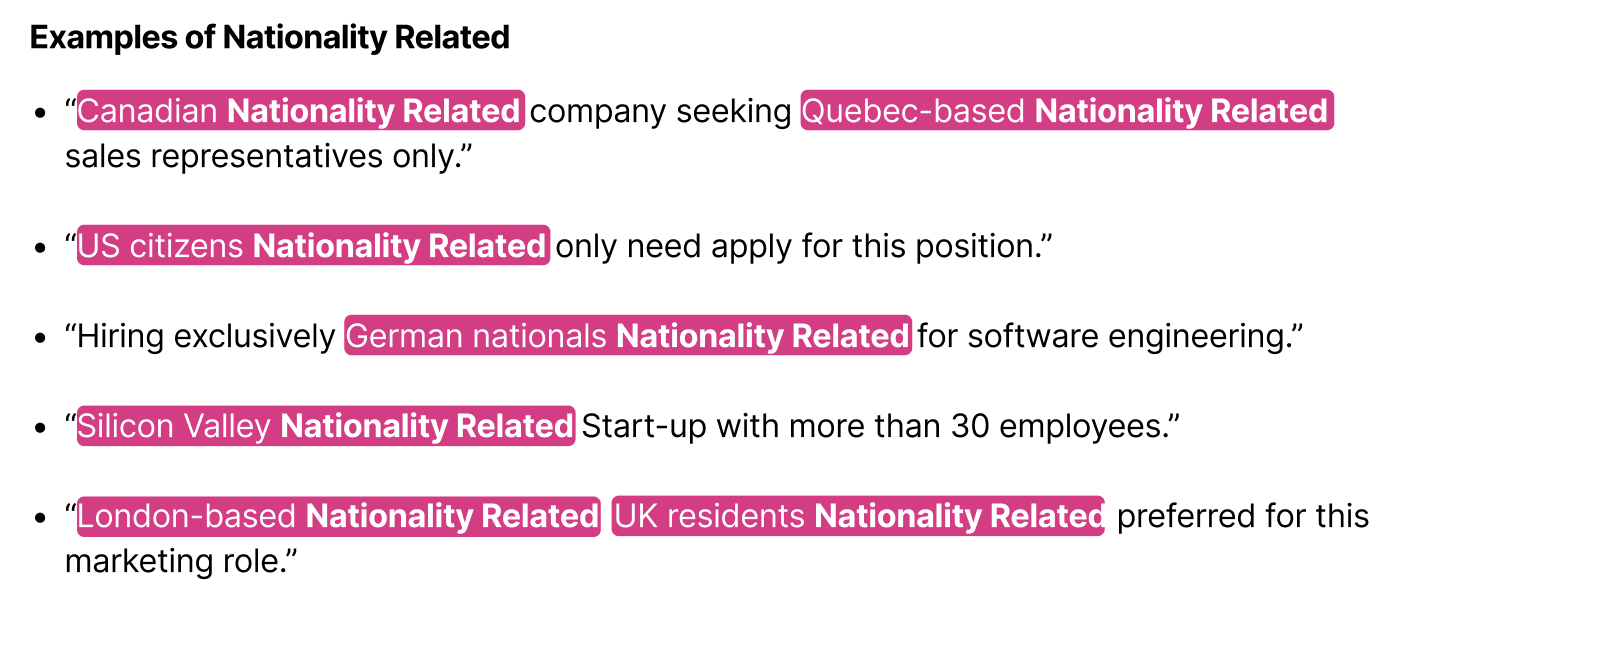
\includegraphics{images/Nationality-Related.png}
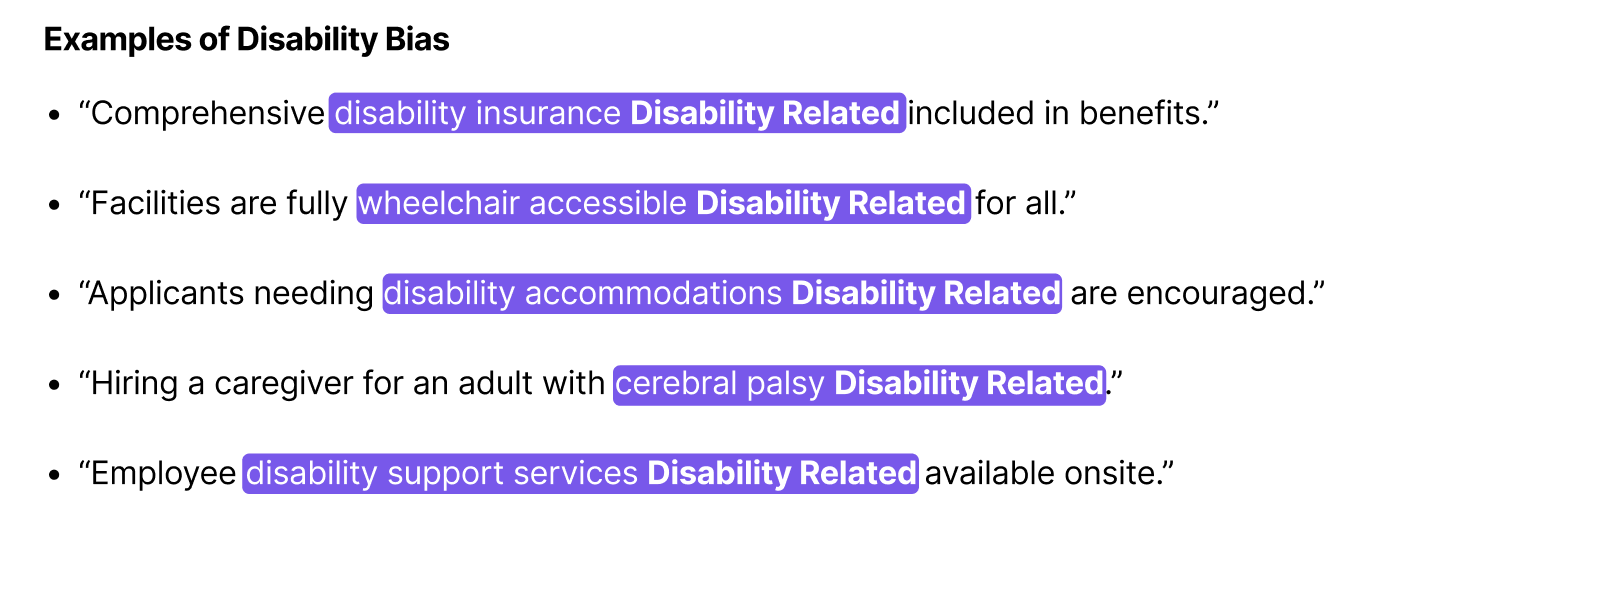
\includegraphics{images/Disability-Related.png}
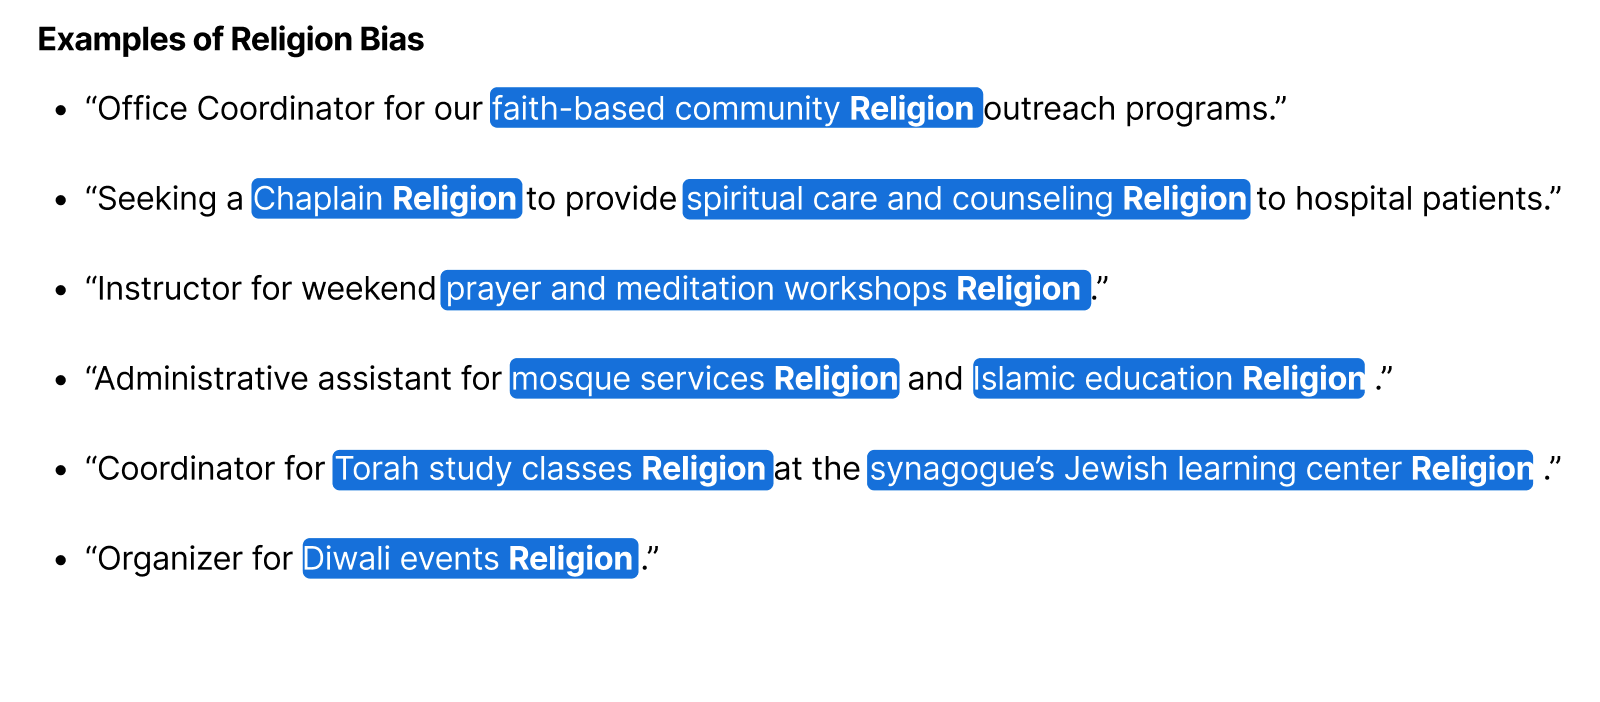
\includegraphics{images/Religion-Related.png}
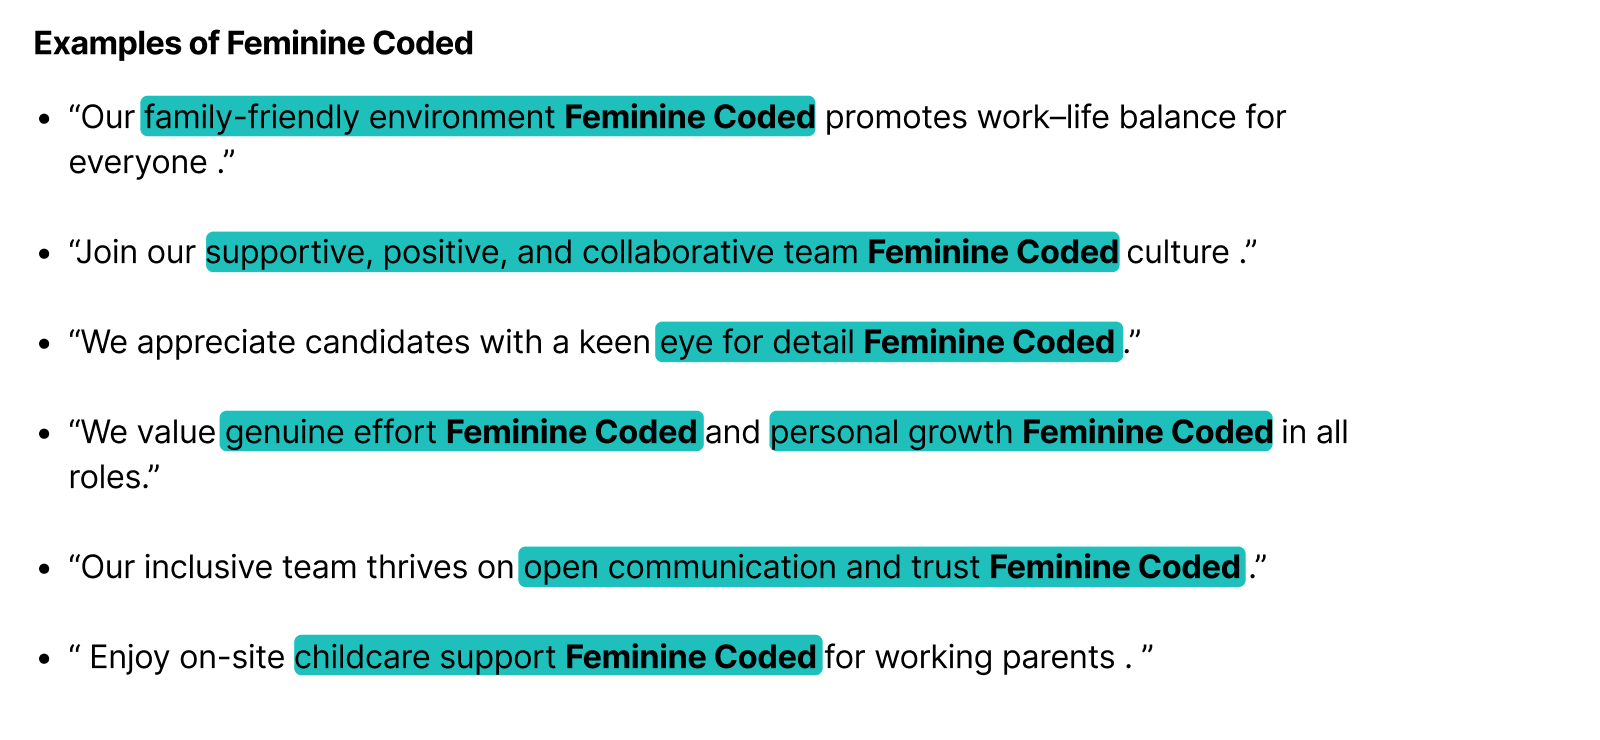
\includegraphics{images/Feminine-Coded.png}

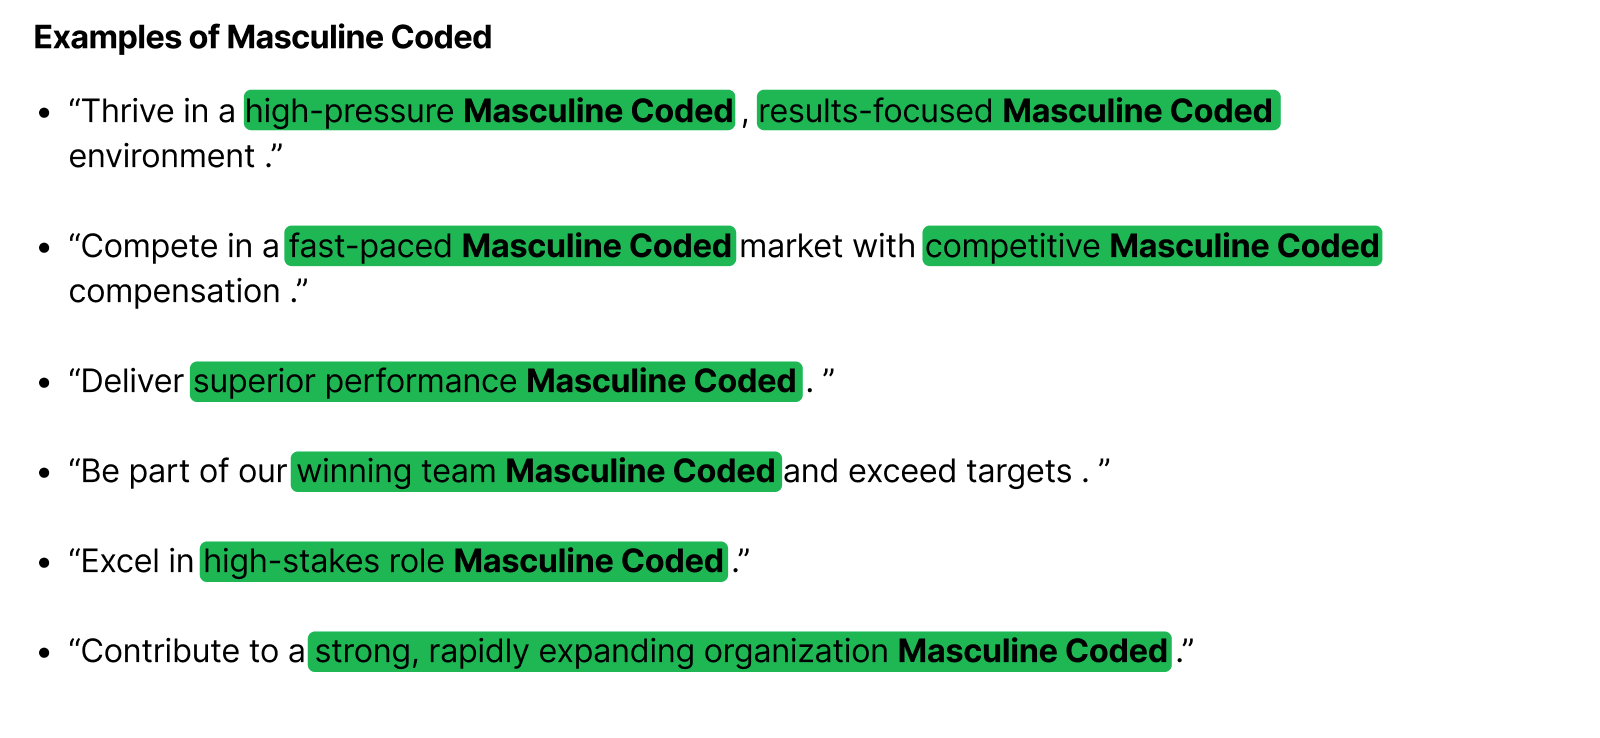
\includegraphics{images/Masculine-Coded.png}
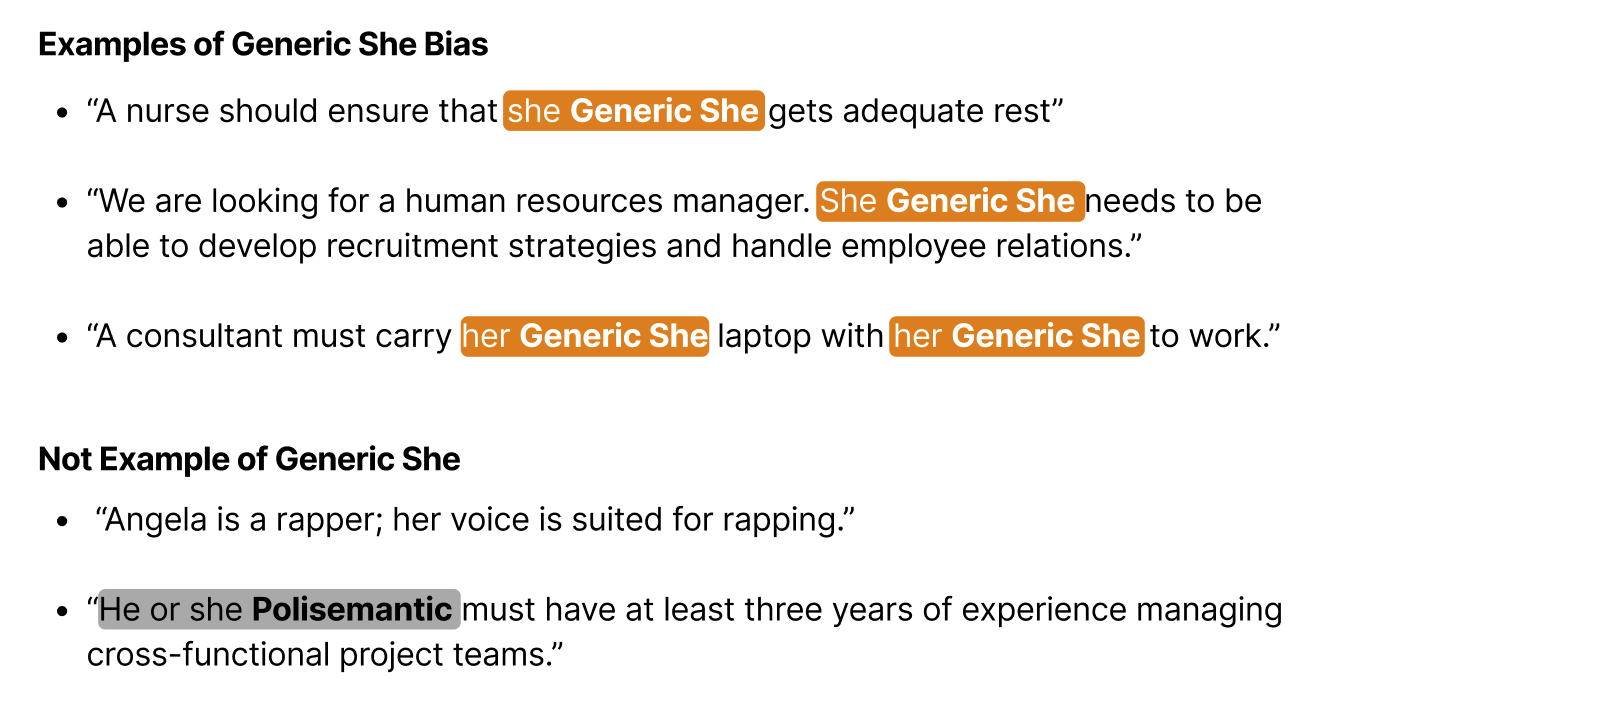
\includegraphics{images/Generic-She.png}
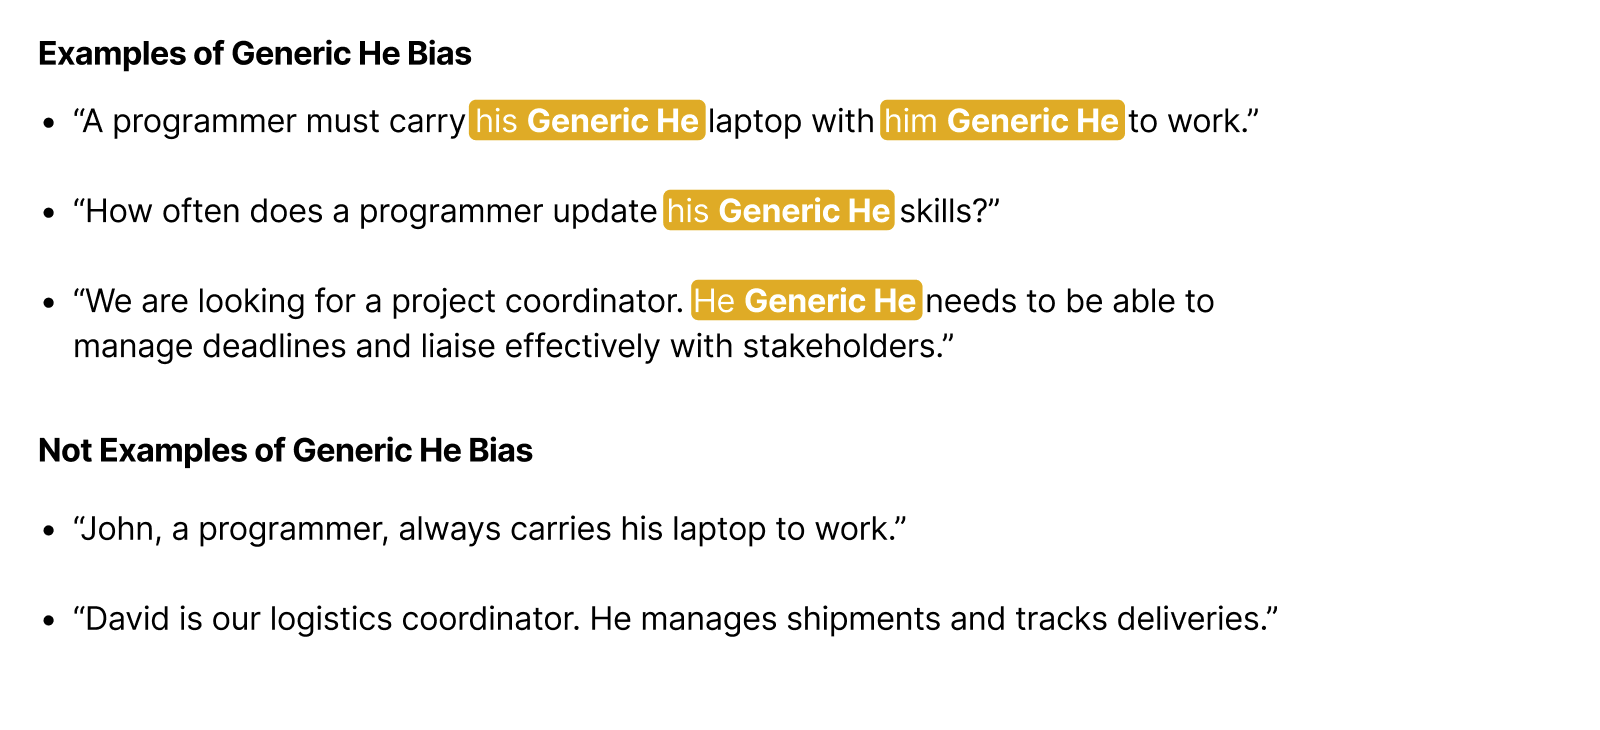
\includegraphics{images/Generic-He.png}
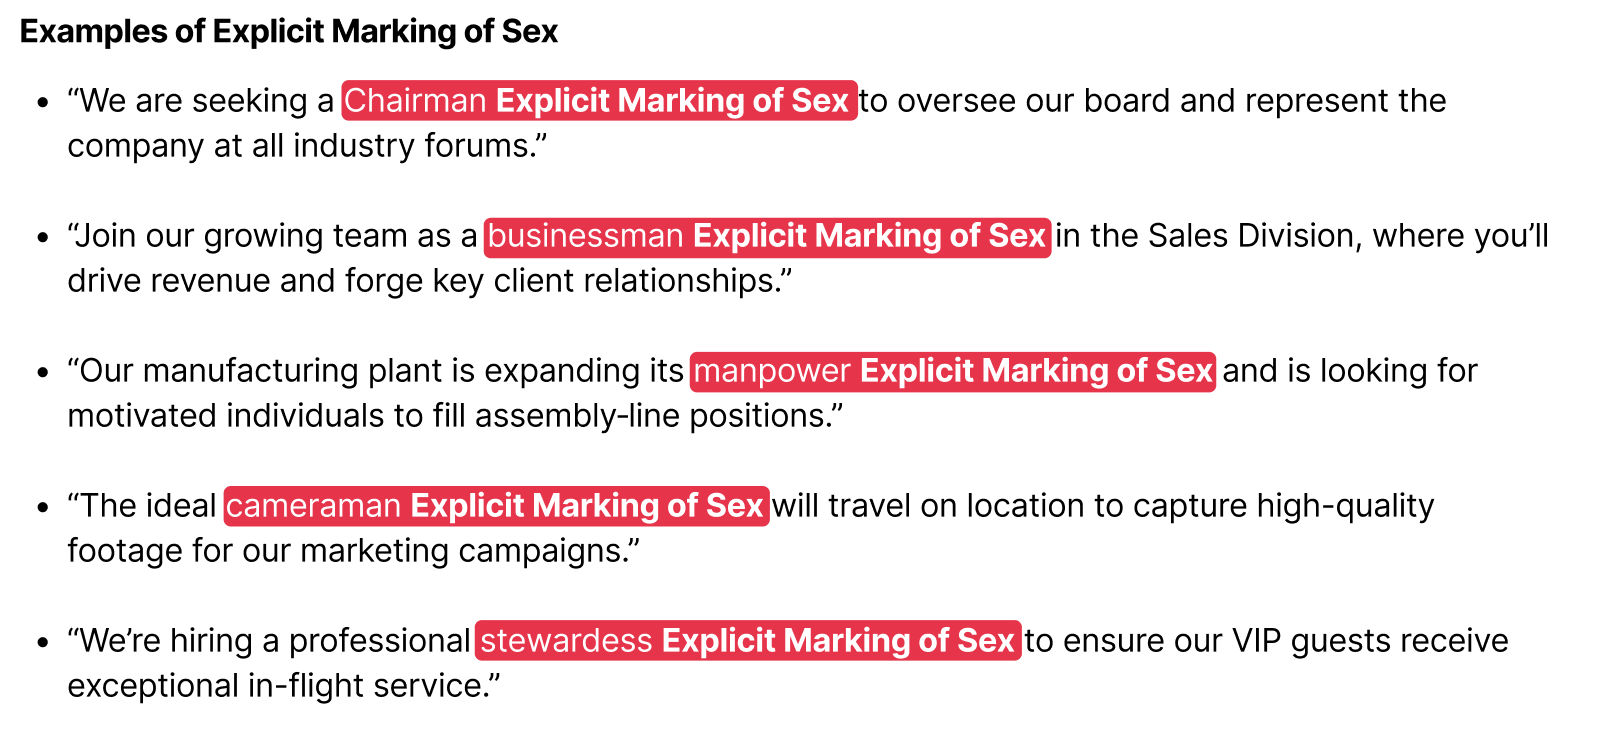
\includegraphics{images/Explicit-Marking.png}
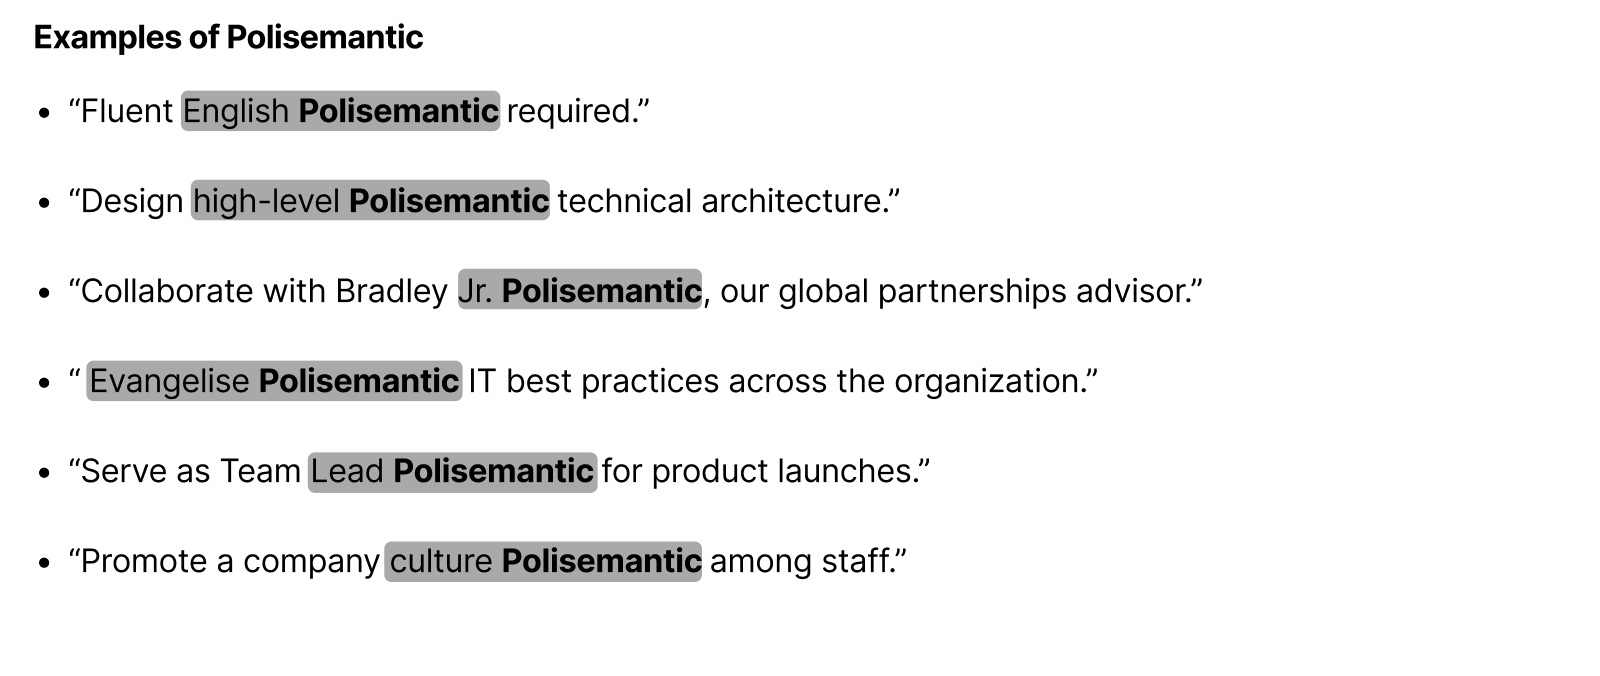
\includegraphics{images/Polisemantic.png}
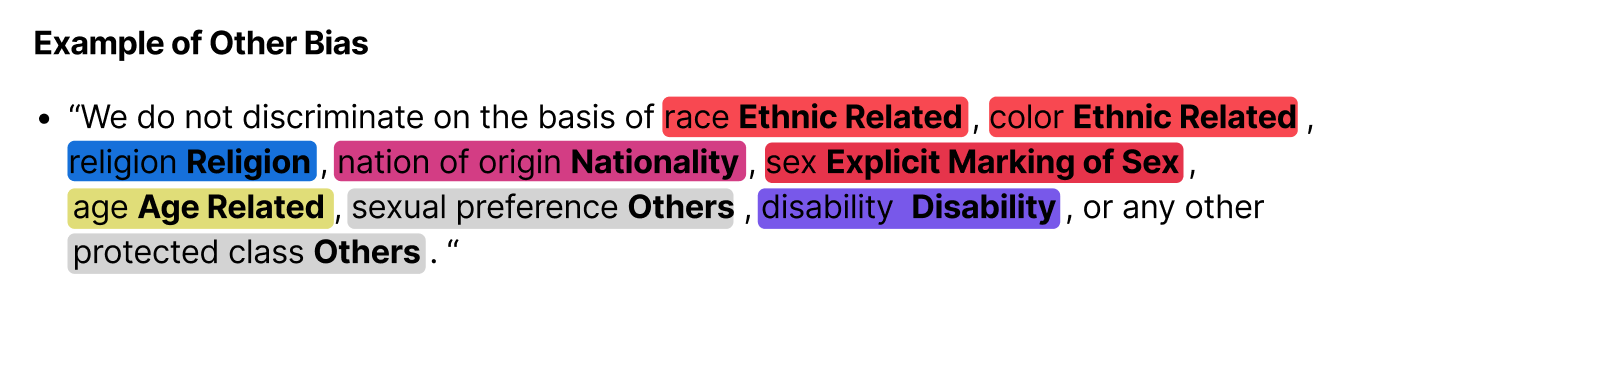
\includegraphics{images/Others.png}

\chapter{References}\label{references}

Bhanumathi, P., Basu, S., \& Babu, B. S. (2024). Artificial intelligence and machine learning- powered recruitment for smart hiring. In Global Practices on Effective Talent Acquisition and Retention (pp.~17--36). \url{https://doi.org/10.4018/979-8-3693-1938-3.ch002}

Born, M. P., Taris, T. W., \& Willemsen, T. M. (2010). ``Perceptions of gender-focused or gender-neutral job advertisements: The effects of job characteristics, communal requirement, and sex of the applicant.'' European Journal of Work and Organizational Psychology, 18(3), 279--305. \url{https://doi.org/10.1080/00224540903365422}

Doughman, J., \& Khreich, W. (2022). Gender bias in text: Labeled datasets and lexicons. ArXiv, abs/2201.08675.

Frissen, R., Adebayo, K. J., \& Nanda, R. (2023). A machine learning approach to recognize bias and discrimination in job advertisements. AI \& Society, 38, 1025--1038. \url{https://doi.org/10.1007/s00146-022-01574-0}

Gaucher, D., Friesen, J., \& Kay, A. C. (2011). Evidence that gendered wording in job advertisements exists and sustains gender inequality. Journal of Personality and Social Psychology, 101(1), 109--128. \url{https://doi.org/10.1037/a0022530}

Heilman, M. E. (2012) ``Gender stereotypes and workplace bias.'' Research in Organizational Behavior, 32, 113--135.https://doi.org/10.1016/j.riob.2012.11.003

Kusner, M. J., Loftus, J. R., Russell, C., \& Silva, R. (2017, March 20). Counterfactual fairness. In Advances in Neural Information Processing Systems, 2017-December (pp.~4067--4077). arXiv.org. \url{https://arxiv.org/abs/1703.06856}

Liu, H., Jin, W., Karimi, H., Liu, Z., \& Tang, J. (2021). The Authors Matter: Understanding and Mitigating Implicit Bias in Deep Text Classification. Association for Computational Linguistics, 74--85. \url{https://aclanthology.org/2021.findings-acl.7.pdf}

Mulkar-Mehta, R., Hobbs, J., \& Hovy, E. (2011). Granularity in natural language discourse. In J. Bos \& S. Pulman (Eds.), Proceedings of the Ninth International Conference on Computational Semantics (IWCS 2011). Association for Computational Linguistics. \url{https://aclanthology.org/W11-0143}

Rudman, L. A., \& Glick, P. (2001). Prescriptive gender stereotypes and backlash toward agentic women. Journal of Social Issues, 57(4), 743--762. \url{https://doi.org/10.1111/0022-} 4537.00239

Schneider, B. (1987). The people make the place. Personnel Psychology, 40(3), 437--453. \url{https://doi.org/10.1111/j.1744-6570.1987.tb00609.x}

Smith, K., Davenport, B. L., Bickford, J. F., Abell, L., \& Dooley, S. (2023). The effects of jargon in STEM job advertisements on genders. Paper presented at the 2023 ASEE Annual Conference \& Exposition, Baltimore, Maryland. \url{https://doi.org/10.18260/1-2--44447}

Tambe, P., Cappelli, P., \& Yakubovich, V. (2019). Artificial intelligence in human resources
management: Challenges and a path forward. California Management Review, 61(4), 15--42. \url{https://doi.org/10.1177/0008125619867910}

\end{document}
